
\documentclass[12pt,a4paper,fleqn]{article}
\usepackage{latexsym,graphicx}
\usepackage[refpage]{nomencl}
\usepackage{../iman,../extra,../isar,../proof}
\usepackage{../isabelle,../isabellesym}
\usepackage{style}
\usepackage{../pdfsetup}

\hyphenation{Isabelle}
\hyphenation{Isar}
\isadroptag{theory}

\title{
\includegraphics[scale=0.5]{isabelle_isar}
  \\[4ex] Code generation from Isabelle/HOL theories}
\author{\emph{Florian Haftmann}}

\begin{document}

\maketitle

\begin{abstract}
  \noindent This tutorial gives an introduction to a generic code generator framework in Isabelle
  for generating executable code in functional programming languages from logical
  specifications in Isabelle/HOL.
\end{abstract}

\thispagestyle{empty}\clearpage

\pagenumbering{roman}
\clearfirst

%
\begin{isabellebody}%
\def\isabellecontext{Introduction}%
%
\isadelimtheory
%
\endisadelimtheory
%
\isatagtheory
\isacommand{theory}\isamarkupfalse%
\ Introduction\isanewline
\isakeyword{imports}\ Setup\isanewline
\isakeyword{begin}%
\endisatagtheory
{\isafoldtheory}%
%
\isadelimtheory
%
\endisadelimtheory
%
\isamarkupchapter{Code generation from \isa{Isabelle{\isacharslash}HOL} theories%
}
\isamarkuptrue%
%
\isamarkupsection{Introduction and Overview%
}
\isamarkuptrue%
%
\begin{isamarkuptext}%
This tutorial introduces a generic code generator for the
  \isa{Isabelle} system.
  Generic in the sense that the
  \qn{target language} for which code shall ultimately be
  generated is not fixed but may be an arbitrary state-of-the-art
  functional programming language (currently, the implementation
  supports \isa{SML} \cite{SML}, \isa{OCaml} \cite{OCaml} and \isa{Haskell}
  \cite{haskell-revised-report}).

  Conceptually the code generator framework is part
  of Isabelle's \hyperlink{theory.Pure}{\mbox{\isa{Pure}}} meta logic framework; the logic
  \hyperlink{theory.HOL}{\mbox{\isa{HOL}}} which is an extension of \hyperlink{theory.Pure}{\mbox{\isa{Pure}}}
  already comes with a reasonable framework setup and thus provides
  a good working horse for raising code-generation-driven
  applications.  So, we assume some familiarity and experience
  with the ingredients of the \hyperlink{theory.HOL}{\mbox{\isa{HOL}}} distribution theories.
  (see also \cite{isa-tutorial}).

  The code generator aims to be usable with no further ado
  in most cases while allowing for detailed customisation.
  This manifests in the structure of this tutorial: after a short
  conceptual introduction with an example (\secref{sec:intro}),
  we discuss the generic customisation facilities (\secref{sec:program}).
  A further section (\secref{sec:adaption}) is dedicated to the matter of
  \qn{adaption} to specific target language environments.  After some
  further issues (\secref{sec:further}) we conclude with an overview
  of some ML programming interfaces (\secref{sec:ml}).

  \begin{warn}
    Ultimately, the code generator which this tutorial deals with
    is supposed to replace the existing code generator
    by Stefan Berghofer \cite{Berghofer-Nipkow:2002}.
    So, for the moment, there are two distinct code generators
    in Isabelle.  In case of ambiguity, we will refer to the framework
    described here as \isa{generic\ code\ generator}, to the
    other as \isa{SML\ code\ generator}.
    Also note that while the framework itself is
    object-logic independent, only \hyperlink{theory.HOL}{\mbox{\isa{HOL}}} provides a reasonable
    framework setup.    
  \end{warn}%
\end{isamarkuptext}%
\isamarkuptrue%
%
\isamarkupsubsection{Code generation via shallow embedding \label{sec:intro}%
}
\isamarkuptrue%
%
\begin{isamarkuptext}%
The key concept for understanding \isa{Isabelle}'s code generation is
  \emph{shallow embedding}, i.e.~logical entities like constants, types and
  classes are identified with corresponding concepts in the target language.

  Inside \hyperlink{theory.HOL}{\mbox{\isa{HOL}}}, the \hyperlink{command.datatype}{\mbox{\isa{\isacommand{datatype}}}} and
  \hyperlink{command.definition}{\mbox{\isa{\isacommand{definition}}}}/\hyperlink{command.primrec}{\mbox{\isa{\isacommand{primrec}}}}/\hyperlink{command.fun}{\mbox{\isa{\isacommand{fun}}}} declarations form
  the core of a functional programming language.  The default code generator setup
  allows to turn those into functional programs immediately.
  This means that \qt{naive} code generation can proceed without further ado.
  For example, here a simple \qt{implementation} of amortised queues:%
\end{isamarkuptext}%
\isamarkuptrue%
%
\isadelimquoteme
%
\endisadelimquoteme
%
\isatagquoteme
\isacommand{datatype}\isamarkupfalse%
\ {\isacharprime}a\ queue\ {\isacharequal}\ Queue\ {\isachardoublequoteopen}{\isacharprime}a\ list{\isachardoublequoteclose}\ {\isachardoublequoteopen}{\isacharprime}a\ list{\isachardoublequoteclose}\isanewline
\isanewline
\isacommand{definition}\isamarkupfalse%
\ empty\ {\isacharcolon}{\isacharcolon}\ {\isachardoublequoteopen}{\isacharprime}a\ queue{\isachardoublequoteclose}\ \isakeyword{where}\isanewline
\ \ {\isachardoublequoteopen}empty\ {\isacharequal}\ Queue\ {\isacharbrackleft}{\isacharbrackright}\ {\isacharbrackleft}{\isacharbrackright}{\isachardoublequoteclose}\isanewline
\isanewline
\isacommand{primrec}\isamarkupfalse%
\ enqueue\ {\isacharcolon}{\isacharcolon}\ {\isachardoublequoteopen}{\isacharprime}a\ {\isasymRightarrow}\ {\isacharprime}a\ queue\ {\isasymRightarrow}\ {\isacharprime}a\ queue{\isachardoublequoteclose}\ \isakeyword{where}\isanewline
\ \ {\isachardoublequoteopen}enqueue\ x\ {\isacharparenleft}Queue\ xs\ ys{\isacharparenright}\ {\isacharequal}\ Queue\ {\isacharparenleft}x\ {\isacharhash}\ xs{\isacharparenright}\ ys{\isachardoublequoteclose}\isanewline
\isanewline
\isacommand{fun}\isamarkupfalse%
\ dequeue\ {\isacharcolon}{\isacharcolon}\ {\isachardoublequoteopen}{\isacharprime}a\ queue\ {\isasymRightarrow}\ {\isacharprime}a\ option\ {\isasymtimes}\ {\isacharprime}a\ queue{\isachardoublequoteclose}\ \isakeyword{where}\isanewline
\ \ \ \ {\isachardoublequoteopen}dequeue\ {\isacharparenleft}Queue\ {\isacharbrackleft}{\isacharbrackright}\ {\isacharbrackleft}{\isacharbrackright}{\isacharparenright}\ {\isacharequal}\ {\isacharparenleft}None{\isacharcomma}\ Queue\ {\isacharbrackleft}{\isacharbrackright}\ {\isacharbrackleft}{\isacharbrackright}{\isacharparenright}{\isachardoublequoteclose}\isanewline
\ \ {\isacharbar}\ {\isachardoublequoteopen}dequeue\ {\isacharparenleft}Queue\ xs\ {\isacharparenleft}y\ {\isacharhash}\ ys{\isacharparenright}{\isacharparenright}\ {\isacharequal}\ {\isacharparenleft}Some\ y{\isacharcomma}\ Queue\ xs\ ys{\isacharparenright}{\isachardoublequoteclose}\isanewline
\ \ {\isacharbar}\ {\isachardoublequoteopen}dequeue\ {\isacharparenleft}Queue\ xs\ {\isacharbrackleft}{\isacharbrackright}{\isacharparenright}\ {\isacharequal}\isanewline
\ \ \ \ \ \ {\isacharparenleft}case\ rev\ xs\ of\ y\ {\isacharhash}\ ys\ {\isasymRightarrow}\ {\isacharparenleft}Some\ y{\isacharcomma}\ Queue\ {\isacharbrackleft}{\isacharbrackright}\ ys{\isacharparenright}{\isacharparenright}{\isachardoublequoteclose}%
\endisatagquoteme
{\isafoldquoteme}%
%
\isadelimquoteme
%
\endisadelimquoteme
%
\begin{isamarkuptext}%
\noindent Then we can generate code e.g.~for \isa{SML} as follows:%
\end{isamarkuptext}%
\isamarkuptrue%
%
\isadelimquoteme
%
\endisadelimquoteme
%
\isatagquoteme
\isacommand{export{\isacharunderscore}code}\isamarkupfalse%
\ empty\ dequeue\ enqueue\ \isakeyword{in}\ SML\isanewline
\ \ \isakeyword{module{\isacharunderscore}name}\ Example\ \isakeyword{file}\ {\isachardoublequoteopen}examples{\isacharslash}example{\isachardot}ML{\isachardoublequoteclose}%
\endisatagquoteme
{\isafoldquoteme}%
%
\isadelimquoteme
%
\endisadelimquoteme
%
\begin{isamarkuptext}%
\noindent resulting in the following code:%
\end{isamarkuptext}%
\isamarkuptrue%
%
\isadelimquoteme
%
\endisadelimquoteme
%
\isatagquoteme
%
\begin{isamarkuptext}%
\isaverbatim%
\noindent%
\verb|structure Example = |\newline%
\verb|struct|\newline%
\newline%
\verb|fun foldl f a [] = a|\newline%
\verb|  |\verb,|,\verb| foldl f a (x :: xs) = foldl f (f a x) xs;|\newline%
\newline%
\verb|fun rev xs = foldl (fn xsa => fn x => x :: xsa) [] xs;|\newline%
\newline%
\verb|fun list_case f1 f2 (a :: lista) = f2 a lista|\newline%
\verb|  |\verb,|,\verb| list_case f1 f2 [] = f1;|\newline%
\newline%
\verb|datatype 'a queue = Queue of 'a list * 'a list;|\newline%
\newline%
\verb|val empty : 'a queue = Queue ([], []);|\newline%
\newline%
\verb|fun dequeue (Queue ([], [])) = (NONE, Queue ([], []))|\newline%
\verb|  |\verb,|,\verb| dequeue (Queue (xs, y :: ys)) = (SOME y, Queue (xs, ys))|\newline%
\verb|  |\verb,|,\verb| dequeue (Queue (v :: va, [])) =|\newline%
\verb|    let|\newline%
\verb|      val y :: ys = rev (v :: va);|\newline%
\verb|    in|\newline%
\verb|      (SOME y, Queue ([], ys))|\newline%
\verb|    end;|\newline%
\newline%
\verb|fun enqueue x (Queue (xs, ys)) = Queue (x :: xs, ys);|\newline%
\newline%
\verb|end; (*struct Example*)|%
\end{isamarkuptext}%
\isamarkuptrue%
%
\endisatagquoteme
{\isafoldquoteme}%
%
\isadelimquoteme
%
\endisadelimquoteme
%
\begin{isamarkuptext}%
\noindent The \hyperlink{command.export-code}{\mbox{\isa{\isacommand{export{\isacharunderscore}code}}}} command takes a space-separated list of
  constants for which code shall be generated;  anything else needed for those
  is added implicitly.  Then follows a target language identifier
  (\isa{SML}, \isa{OCaml} or \isa{Haskell}) and a freely chosen module name.
  A file name denotes the destination to store the generated code.  Note that
  the semantics of the destination depends on the target language:  for
  \isa{SML} and \isa{OCaml} it denotes a \emph{file}, for \isa{Haskell}
  it denotes a \emph{directory} where a file named as the module name
  (with extension \isa{{\isachardot}hs}) is written:%
\end{isamarkuptext}%
\isamarkuptrue%
%
\isadelimquoteme
%
\endisadelimquoteme
%
\isatagquoteme
\isacommand{export{\isacharunderscore}code}\isamarkupfalse%
\ empty\ dequeue\ enqueue\ \isakeyword{in}\ Haskell\isanewline
\ \ \isakeyword{module{\isacharunderscore}name}\ Example\ \isakeyword{file}\ {\isachardoublequoteopen}examples{\isacharslash}{\isachardoublequoteclose}%
\endisatagquoteme
{\isafoldquoteme}%
%
\isadelimquoteme
%
\endisadelimquoteme
%
\begin{isamarkuptext}%
\noindent This is how the corresponding code in \isa{Haskell} looks like:%
\end{isamarkuptext}%
\isamarkuptrue%
%
\isadelimquoteme
%
\endisadelimquoteme
%
\isatagquoteme
%
\begin{isamarkuptext}%
\isaverbatim%
\noindent%
\verb|module Example where {|\newline%
\newline%
\newline%
\verb|foldla :: forall a b. (a -> b -> a) -> a -> [b] -> a;|\newline%
\verb|foldla f a [] = a;|\newline%
\verb|foldla f a (x : xs) = foldla f (f a x) xs;|\newline%
\newline%
\verb|rev :: forall a. [a] -> [a];|\newline%
\verb|rev xs = foldla (\ xsa x -> x : xsa) [] xs;|\newline%
\newline%
\verb|list_case :: forall t a. t -> (a -> [a] -> t) -> [a] -> t;|\newline%
\verb|list_case f1 f2 (a : list) = f2 a list;|\newline%
\verb|list_case f1 f2 [] = f1;|\newline%
\newline%
\verb|data Queue a = Queue [a] [a];|\newline%
\newline%
\verb|empty :: forall a. Queue a;|\newline%
\verb|empty = Queue [] [];|\newline%
\newline%
\verb|dequeue :: forall a. Queue a -> (Maybe a, Queue a);|\newline%
\verb|dequeue (Queue [] []) = (Nothing, Queue [] []);|\newline%
\verb|dequeue (Queue xs (y : ys)) = (Just y, Queue xs ys);|\newline%
\verb|dequeue (Queue (v : va) []) =|\newline%
\verb|  let {|\newline%
\verb|    (y : ys) = rev (v : va);|\newline%
\verb|  } in (Just y, Queue [] ys);|\newline%
\newline%
\verb|enqueue :: forall a. a -> Queue a -> Queue a;|\newline%
\verb|enqueue x (Queue xs ys) = Queue (x : xs) ys;|\newline%
\newline%
\verb|}|%
\end{isamarkuptext}%
\isamarkuptrue%
%
\endisatagquoteme
{\isafoldquoteme}%
%
\isadelimquoteme
%
\endisadelimquoteme
%
\begin{isamarkuptext}%
\noindent This demonstrates the basic usage of the \hyperlink{command.export-code}{\mbox{\isa{\isacommand{export{\isacharunderscore}code}}}} command;
  for more details see \secref{sec:further}.%
\end{isamarkuptext}%
\isamarkuptrue%
%
\isamarkupsubsection{Code generator architecture \label{sec:concept}%
}
\isamarkuptrue%
%
\begin{isamarkuptext}%
What you have seen so far should be already enough in a lot of cases.  If you
  are content with this, you can quit reading here.  Anyway, in order to customise
  and adapt the code generator, it is inevitable to gain some understanding
  how it works.

  \begin{figure}[h]
    \centering
    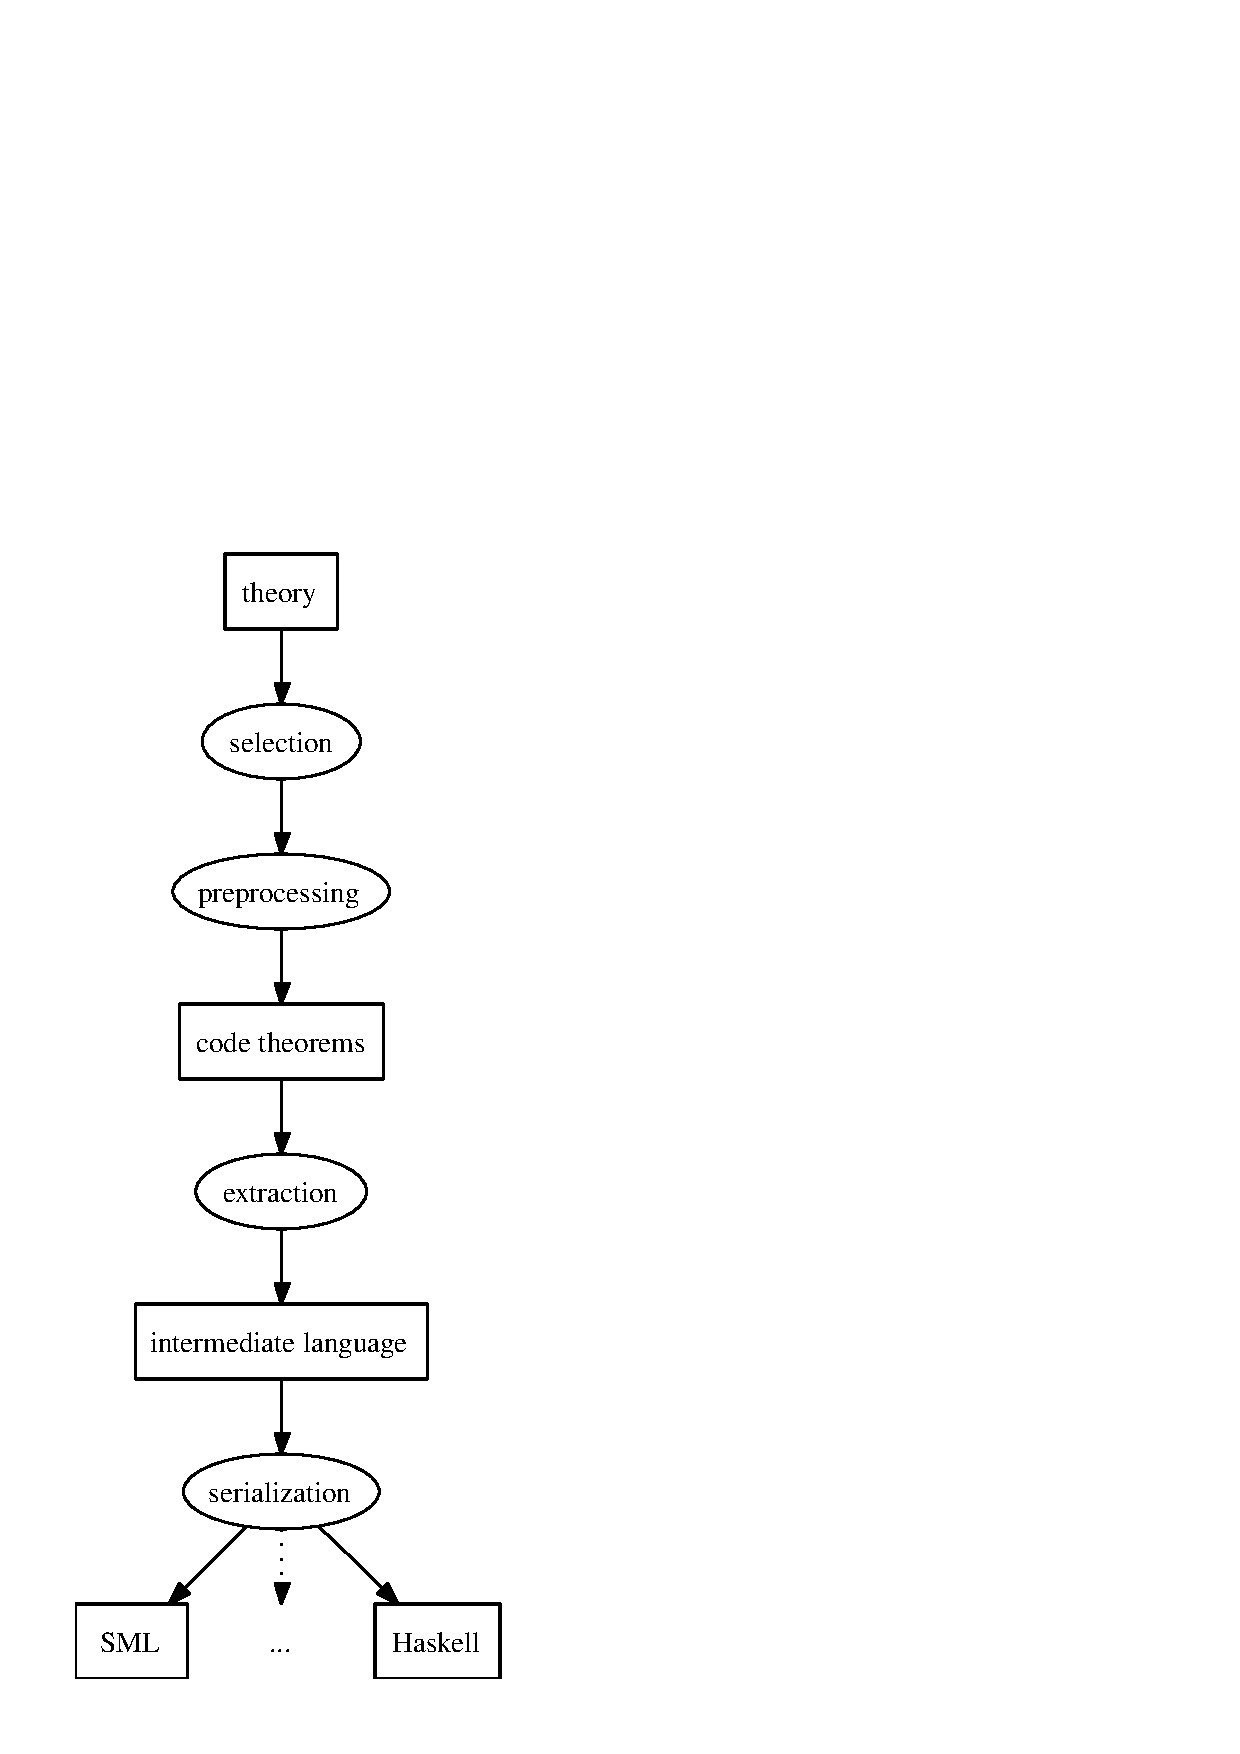
\includegraphics[width=0.7\textwidth]{codegen_process}
    \caption{Code generator architecture}
    \label{fig:arch}
  \end{figure}

  The code generator employs a notion of executability
  for three foundational executable ingredients known
  from functional programming:
  \emph{defining equations}, \emph{datatypes}, and
  \emph{type classes}.  A defining equation as a first approximation
  is a theorem of the form \isa{f\ t\isactrlisub {\isadigit{1}}\ t\isactrlisub {\isadigit{2}}\ {\isasymdots}\ t\isactrlisub n\ {\isasymequiv}\ t}
  (an equation headed by a constant \isa{f} with arguments
  \isa{t\isactrlisub {\isadigit{1}}\ t\isactrlisub {\isadigit{2}}\ {\isasymdots}\ t\isactrlisub n} and right hand side \isa{t}).
  Code generation aims to turn defining equations
  into a functional program.  This is achieved by three major
  components which operate sequentially, i.e. the result of one is
  the input
  of the next in the chain,  see diagram \ref{fig:arch}:

  \begin{itemize}

    \item Out of the vast collection of theorems proven in a
      \qn{theory}, a reasonable subset modelling
      defining equations is \qn{selected}.

    \item On those selected theorems, certain
      transformations are carried out
      (\qn{preprocessing}).  Their purpose is to turn theorems
      representing non- or badly executable
      specifications into equivalent but executable counterparts.
      The result is a structured collection of \qn{code theorems}.

    \item Before the selected defining equations are continued with,
      they can be \qn{preprocessed}, i.e. subjected to theorem
      transformations.  This \qn{preprocessor} is an interface which
      allows to apply
      the full expressiveness of ML-based theorem transformations
      to code generation;  motivating examples are shown below, see
      \secref{sec:preproc}.
      The result of the preprocessing step is a structured collection
      of defining equations.

    \item These defining equations are \qn{translated} to a program
      in an abstract intermediate language.  Think of it as a kind
      of \qt{Mini-Haskell} with four \qn{statements}: \isa{data}
      (for datatypes), \isa{fun} (stemming from defining equations),
      also \isa{class} and \isa{inst} (for type classes).

    \item Finally, the abstract program is \qn{serialised} into concrete
      source code of a target language.

  \end{itemize}

  \noindent From these steps, only the two last are carried out outside the logic;  by
  keeping this layer as thin as possible, the amount of code to trust is
  kept to a minimum.%
\end{isamarkuptext}%
\isamarkuptrue%
%
\isadelimtheory
%
\endisadelimtheory
%
\isatagtheory
\isacommand{end}\isamarkupfalse%
%
\endisatagtheory
{\isafoldtheory}%
%
\isadelimtheory
%
\endisadelimtheory
\isanewline
\end{isabellebody}%
%%% Local Variables:
%%% mode: latex
%%% TeX-master: "root"
%%% End:

%
\begin{isabellebody}%
\def\isabellecontext{Program}%
%
\isadelimtheory
%
\endisadelimtheory
%
\isatagtheory
\isacommand{theory}\isamarkupfalse%
\ Program\isanewline
\isakeyword{imports}\ Introduction\isanewline
\isakeyword{begin}%
\endisatagtheory
{\isafoldtheory}%
%
\isadelimtheory
%
\endisadelimtheory
%
\isamarkupsection{Turning Theories into Programs \label{sec:program}%
}
\isamarkuptrue%
%
\isamarkupsubsection{The \isa{Isabelle{\isacharslash}HOL} default setup%
}
\isamarkuptrue%
%
\begin{isamarkuptext}%
We have already seen how by default equations stemming from
  \hyperlink{command.definition}{\mbox{\isa{\isacommand{definition}}}}/\hyperlink{command.primrec}{\mbox{\isa{\isacommand{primrec}}}}/\hyperlink{command.fun}{\mbox{\isa{\isacommand{fun}}}}
  statements are used for code generation.  This default behaviour
  can be changed, e.g. by providing different code equations.
  All kinds of customisation shown in this section is \emph{safe}
  in the sense that the user does not have to worry about
  correctness -- all programs generatable that way are partially
  correct.%
\end{isamarkuptext}%
\isamarkuptrue%
%
\isamarkupsubsection{Selecting code equations%
}
\isamarkuptrue%
%
\begin{isamarkuptext}%
Coming back to our introductory example, we
  could provide an alternative code equations for \isa{dequeue}
  explicitly:%
\end{isamarkuptext}%
\isamarkuptrue%
%
\isadelimquote
%
\endisadelimquote
%
\isatagquote
\isacommand{lemma}\isamarkupfalse%
\ {\isacharbrackleft}code{\isacharbrackright}{\isacharcolon}\isanewline
\ \ {\isachardoublequoteopen}dequeue\ {\isacharparenleft}AQueue\ xs\ {\isacharbrackleft}{\isacharbrackright}{\isacharparenright}\ {\isacharequal}\isanewline
\ \ \ \ \ {\isacharparenleft}if\ xs\ {\isacharequal}\ {\isacharbrackleft}{\isacharbrackright}\ then\ {\isacharparenleft}None{\isacharcomma}\ AQueue\ {\isacharbrackleft}{\isacharbrackright}\ {\isacharbrackleft}{\isacharbrackright}{\isacharparenright}\isanewline
\ \ \ \ \ \ \ else\ dequeue\ {\isacharparenleft}AQueue\ {\isacharbrackleft}{\isacharbrackright}\ {\isacharparenleft}rev\ xs{\isacharparenright}{\isacharparenright}{\isacharparenright}{\isachardoublequoteclose}\isanewline
\ \ {\isachardoublequoteopen}dequeue\ {\isacharparenleft}AQueue\ xs\ {\isacharparenleft}y\ {\isacharhash}\ ys{\isacharparenright}{\isacharparenright}\ {\isacharequal}\isanewline
\ \ \ \ \ {\isacharparenleft}Some\ y{\isacharcomma}\ AQueue\ xs\ ys{\isacharparenright}{\isachardoublequoteclose}\isanewline
\ \ \isacommand{by}\isamarkupfalse%
\ {\isacharparenleft}cases\ xs{\isacharcomma}\ simp{\isacharunderscore}all{\isacharparenright}\ {\isacharparenleft}cases\ {\isachardoublequoteopen}rev\ xs{\isachardoublequoteclose}{\isacharcomma}\ simp{\isacharunderscore}all{\isacharparenright}%
\endisatagquote
{\isafoldquote}%
%
\isadelimquote
%
\endisadelimquote
%
\begin{isamarkuptext}%
\noindent The annotation \isa{{\isacharbrackleft}code{\isacharbrackright}} is an \isa{Isar}
  \isa{attribute} which states that the given theorems should be
  considered as code equations for a \isa{fun} statement --
  the corresponding constant is determined syntactically.  The resulting code:%
\end{isamarkuptext}%
\isamarkuptrue%
%
\isadelimquote
%
\endisadelimquote
%
\isatagquote
%
\begin{isamarkuptext}%
\isatypewriter%
\noindent%
\hspace*{0pt}dequeue ::~forall a.~Queue a -> (Maybe a,~Queue a);\\
\hspace*{0pt}dequeue (AQueue xs (y :~ys)) = (Just y,~AQueue xs ys);\\
\hspace*{0pt}dequeue (AQueue xs []) =\\
\hspace*{0pt} ~(if nulla xs then (Nothing,~AQueue [] [])\\
\hspace*{0pt} ~~~else dequeue (AQueue [] (rev xs)));%
\end{isamarkuptext}%
\isamarkuptrue%
%
\endisatagquote
{\isafoldquote}%
%
\isadelimquote
%
\endisadelimquote
%
\begin{isamarkuptext}%
\noindent You may note that the equality test \isa{xs\ {\isacharequal}\ {\isacharbrackleft}{\isacharbrackright}} has been
  replaced by the predicate \isa{null\ xs}.  This is due to the default
  setup in the \qn{preprocessor} to be discussed further below (\secref{sec:preproc}).

  Changing the default constructor set of datatypes is also
  possible.  See \secref{sec:datatypes} for an example.

  As told in \secref{sec:concept}, code generation is based
  on a structured collection of code theorems.
  For explorative purpose, this collection
  may be inspected using the \hyperlink{command.code-thms}{\mbox{\isa{\isacommand{code{\isacharunderscore}thms}}}} command:%
\end{isamarkuptext}%
\isamarkuptrue%
%
\isadelimquote
%
\endisadelimquote
%
\isatagquote
\isacommand{code{\isacharunderscore}thms}\isamarkupfalse%
\ dequeue%
\endisatagquote
{\isafoldquote}%
%
\isadelimquote
%
\endisadelimquote
%
\begin{isamarkuptext}%
\noindent prints a table with \emph{all} code equations
  for \isa{dequeue}, including
  \emph{all} code equations those equations depend
  on recursively.
  
  Similarly, the \hyperlink{command.code-deps}{\mbox{\isa{\isacommand{code{\isacharunderscore}deps}}}} command shows a graph
  visualising dependencies between code equations.%
\end{isamarkuptext}%
\isamarkuptrue%
%
\isamarkupsubsection{\isa{class} and \isa{instantiation}%
}
\isamarkuptrue%
%
\begin{isamarkuptext}%
Concerning type classes and code generation, let us examine an example
  from abstract algebra:%
\end{isamarkuptext}%
\isamarkuptrue%
%
\isadelimquote
%
\endisadelimquote
%
\isatagquote
\isacommand{class}\isamarkupfalse%
\ semigroup\ {\isacharequal}\isanewline
\ \ \isakeyword{fixes}\ mult\ {\isacharcolon}{\isacharcolon}\ {\isachardoublequoteopen}{\isacharprime}a\ {\isasymRightarrow}\ {\isacharprime}a\ {\isasymRightarrow}\ {\isacharprime}a{\isachardoublequoteclose}\ {\isacharparenleft}\isakeyword{infixl}\ {\isachardoublequoteopen}{\isasymotimes}{\isachardoublequoteclose}\ {\isadigit{7}}{\isadigit{0}}{\isacharparenright}\isanewline
\ \ \isakeyword{assumes}\ assoc{\isacharcolon}\ {\isachardoublequoteopen}{\isacharparenleft}x\ {\isasymotimes}\ y{\isacharparenright}\ {\isasymotimes}\ z\ {\isacharequal}\ x\ {\isasymotimes}\ {\isacharparenleft}y\ {\isasymotimes}\ z{\isacharparenright}{\isachardoublequoteclose}\isanewline
\isanewline
\isacommand{class}\isamarkupfalse%
\ monoid\ {\isacharequal}\ semigroup\ {\isacharplus}\isanewline
\ \ \isakeyword{fixes}\ neutral\ {\isacharcolon}{\isacharcolon}\ {\isacharprime}a\ {\isacharparenleft}{\isachardoublequoteopen}{\isasymone}{\isachardoublequoteclose}{\isacharparenright}\isanewline
\ \ \isakeyword{assumes}\ neutl{\isacharcolon}\ {\isachardoublequoteopen}{\isasymone}\ {\isasymotimes}\ x\ {\isacharequal}\ x{\isachardoublequoteclose}\isanewline
\ \ \ \ \isakeyword{and}\ neutr{\isacharcolon}\ {\isachardoublequoteopen}x\ {\isasymotimes}\ {\isasymone}\ {\isacharequal}\ x{\isachardoublequoteclose}\isanewline
\isanewline
\isacommand{instantiation}\isamarkupfalse%
\ nat\ {\isacharcolon}{\isacharcolon}\ monoid\isanewline
\isakeyword{begin}\isanewline
\isanewline
\isacommand{primrec}\isamarkupfalse%
\ mult{\isacharunderscore}nat\ \isakeyword{where}\isanewline
\ \ \ \ {\isachardoublequoteopen}{\isadigit{0}}\ {\isasymotimes}\ n\ {\isacharequal}\ {\isacharparenleft}{\isadigit{0}}{\isasymColon}nat{\isacharparenright}{\isachardoublequoteclose}\isanewline
\ \ {\isacharbar}\ {\isachardoublequoteopen}Suc\ m\ {\isasymotimes}\ n\ {\isacharequal}\ n\ {\isacharplus}\ m\ {\isasymotimes}\ n{\isachardoublequoteclose}\isanewline
\isanewline
\isacommand{definition}\isamarkupfalse%
\ neutral{\isacharunderscore}nat\ \isakeyword{where}\isanewline
\ \ {\isachardoublequoteopen}{\isasymone}\ {\isacharequal}\ Suc\ {\isadigit{0}}{\isachardoublequoteclose}\isanewline
\isanewline
\isacommand{lemma}\isamarkupfalse%
\ add{\isacharunderscore}mult{\isacharunderscore}distrib{\isacharcolon}\isanewline
\ \ \isakeyword{fixes}\ n\ m\ q\ {\isacharcolon}{\isacharcolon}\ nat\isanewline
\ \ \isakeyword{shows}\ {\isachardoublequoteopen}{\isacharparenleft}n\ {\isacharplus}\ m{\isacharparenright}\ {\isasymotimes}\ q\ {\isacharequal}\ n\ {\isasymotimes}\ q\ {\isacharplus}\ m\ {\isasymotimes}\ q{\isachardoublequoteclose}\isanewline
\ \ \isacommand{by}\isamarkupfalse%
\ {\isacharparenleft}induct\ n{\isacharparenright}\ simp{\isacharunderscore}all\isanewline
\isanewline
\isacommand{instance}\isamarkupfalse%
\ \isacommand{proof}\isamarkupfalse%
\isanewline
\ \ \isacommand{fix}\isamarkupfalse%
\ m\ n\ q\ {\isacharcolon}{\isacharcolon}\ nat\isanewline
\ \ \isacommand{show}\isamarkupfalse%
\ {\isachardoublequoteopen}m\ {\isasymotimes}\ n\ {\isasymotimes}\ q\ {\isacharequal}\ m\ {\isasymotimes}\ {\isacharparenleft}n\ {\isasymotimes}\ q{\isacharparenright}{\isachardoublequoteclose}\isanewline
\ \ \ \ \isacommand{by}\isamarkupfalse%
\ {\isacharparenleft}induct\ m{\isacharparenright}\ {\isacharparenleft}simp{\isacharunderscore}all\ add{\isacharcolon}\ add{\isacharunderscore}mult{\isacharunderscore}distrib{\isacharparenright}\isanewline
\ \ \isacommand{show}\isamarkupfalse%
\ {\isachardoublequoteopen}{\isasymone}\ {\isasymotimes}\ n\ {\isacharequal}\ n{\isachardoublequoteclose}\isanewline
\ \ \ \ \isacommand{by}\isamarkupfalse%
\ {\isacharparenleft}simp\ add{\isacharcolon}\ neutral{\isacharunderscore}nat{\isacharunderscore}def{\isacharparenright}\isanewline
\ \ \isacommand{show}\isamarkupfalse%
\ {\isachardoublequoteopen}m\ {\isasymotimes}\ {\isasymone}\ {\isacharequal}\ m{\isachardoublequoteclose}\isanewline
\ \ \ \ \isacommand{by}\isamarkupfalse%
\ {\isacharparenleft}induct\ m{\isacharparenright}\ {\isacharparenleft}simp{\isacharunderscore}all\ add{\isacharcolon}\ neutral{\isacharunderscore}nat{\isacharunderscore}def{\isacharparenright}\isanewline
\isacommand{qed}\isamarkupfalse%
\isanewline
\isanewline
\isacommand{end}\isamarkupfalse%
%
\endisatagquote
{\isafoldquote}%
%
\isadelimquote
%
\endisadelimquote
%
\begin{isamarkuptext}%
\noindent We define the natural operation of the natural numbers
  on monoids:%
\end{isamarkuptext}%
\isamarkuptrue%
%
\isadelimquote
%
\endisadelimquote
%
\isatagquote
\isacommand{primrec}\isamarkupfalse%
\ {\isacharparenleft}\isakeyword{in}\ monoid{\isacharparenright}\ pow\ {\isacharcolon}{\isacharcolon}\ {\isachardoublequoteopen}nat\ {\isasymRightarrow}\ {\isacharprime}a\ {\isasymRightarrow}\ {\isacharprime}a{\isachardoublequoteclose}\ \isakeyword{where}\isanewline
\ \ \ \ {\isachardoublequoteopen}pow\ {\isadigit{0}}\ a\ {\isacharequal}\ {\isasymone}{\isachardoublequoteclose}\isanewline
\ \ {\isacharbar}\ {\isachardoublequoteopen}pow\ {\isacharparenleft}Suc\ n{\isacharparenright}\ a\ {\isacharequal}\ a\ {\isasymotimes}\ pow\ n\ a{\isachardoublequoteclose}%
\endisatagquote
{\isafoldquote}%
%
\isadelimquote
%
\endisadelimquote
%
\begin{isamarkuptext}%
\noindent This we use to define the discrete exponentiation function:%
\end{isamarkuptext}%
\isamarkuptrue%
%
\isadelimquote
%
\endisadelimquote
%
\isatagquote
\isacommand{definition}\isamarkupfalse%
\ bexp\ {\isacharcolon}{\isacharcolon}\ {\isachardoublequoteopen}nat\ {\isasymRightarrow}\ nat{\isachardoublequoteclose}\ \isakeyword{where}\isanewline
\ \ {\isachardoublequoteopen}bexp\ n\ {\isacharequal}\ pow\ n\ {\isacharparenleft}Suc\ {\isacharparenleft}Suc\ {\isadigit{0}}{\isacharparenright}{\isacharparenright}{\isachardoublequoteclose}%
\endisatagquote
{\isafoldquote}%
%
\isadelimquote
%
\endisadelimquote
%
\begin{isamarkuptext}%
\noindent The corresponding code:%
\end{isamarkuptext}%
\isamarkuptrue%
%
\isadelimquote
%
\endisadelimquote
%
\isatagquote
%
\begin{isamarkuptext}%
\isatypewriter%
\noindent%
\hspace*{0pt}module Example where {\char123}\\
\hspace*{0pt}\\
\hspace*{0pt}\\
\hspace*{0pt}data Nat = Zero{\char95}nat | Suc Nat;\\
\hspace*{0pt}\\
\hspace*{0pt}class Semigroup a where {\char123}\\
\hspace*{0pt} ~mult ::~a -> a -> a;\\
\hspace*{0pt}{\char125};\\
\hspace*{0pt}\\
\hspace*{0pt}class (Semigroup a) => Monoid a where {\char123}\\
\hspace*{0pt} ~neutral ::~a;\\
\hspace*{0pt}{\char125};\\
\hspace*{0pt}\\
\hspace*{0pt}pow ::~forall a.~(Monoid a) => Nat -> a -> a;\\
\hspace*{0pt}pow Zero{\char95}nat a = neutral;\\
\hspace*{0pt}pow (Suc n) a = mult a (pow n a);\\
\hspace*{0pt}\\
\hspace*{0pt}plus{\char95}nat ::~Nat -> Nat -> Nat;\\
\hspace*{0pt}plus{\char95}nat (Suc m) n = plus{\char95}nat m (Suc n);\\
\hspace*{0pt}plus{\char95}nat Zero{\char95}nat n = n;\\
\hspace*{0pt}\\
\hspace*{0pt}neutral{\char95}nat ::~Nat;\\
\hspace*{0pt}neutral{\char95}nat = Suc Zero{\char95}nat;\\
\hspace*{0pt}\\
\hspace*{0pt}mult{\char95}nat ::~Nat -> Nat -> Nat;\\
\hspace*{0pt}mult{\char95}nat Zero{\char95}nat n = Zero{\char95}nat;\\
\hspace*{0pt}mult{\char95}nat (Suc m) n = plus{\char95}nat n (mult{\char95}nat m n);\\
\hspace*{0pt}\\
\hspace*{0pt}instance Semigroup Nat where {\char123}\\
\hspace*{0pt} ~mult = mult{\char95}nat;\\
\hspace*{0pt}{\char125};\\
\hspace*{0pt}\\
\hspace*{0pt}instance Monoid Nat where {\char123}\\
\hspace*{0pt} ~neutral = neutral{\char95}nat;\\
\hspace*{0pt}{\char125};\\
\hspace*{0pt}\\
\hspace*{0pt}bexp ::~Nat -> Nat;\\
\hspace*{0pt}bexp n = pow n (Suc (Suc Zero{\char95}nat));\\
\hspace*{0pt}\\
\hspace*{0pt}{\char125}%
\end{isamarkuptext}%
\isamarkuptrue%
%
\endisatagquote
{\isafoldquote}%
%
\isadelimquote
%
\endisadelimquote
%
\begin{isamarkuptext}%
\noindent This is a convenient place to show how explicit dictionary construction
  manifests in generated code (here, the same example in \isa{SML}):%
\end{isamarkuptext}%
\isamarkuptrue%
%
\isadelimquote
%
\endisadelimquote
%
\isatagquote
%
\begin{isamarkuptext}%
\isatypewriter%
\noindent%
\hspace*{0pt}structure Example = \\
\hspace*{0pt}struct\\
\hspace*{0pt}\\
\hspace*{0pt}datatype nat = Zero{\char95}nat | Suc of nat;\\
\hspace*{0pt}\\
\hspace*{0pt}type 'a semigroup = {\char123}mult :~'a -> 'a -> 'a{\char125};\\
\hspace*{0pt}fun mult (A{\char95}:'a semigroup) = {\char35}mult A{\char95};\\
\hspace*{0pt}\\
\hspace*{0pt}type 'a monoid = {\char123}Program{\char95}{\char95}semigroup{\char95}monoid :~'a semigroup,~neutral :~'a{\char125};\\
\hspace*{0pt}fun semigroup{\char95}monoid (A{\char95}:'a monoid) = {\char35}Program{\char95}{\char95}semigroup{\char95}monoid A{\char95};\\
\hspace*{0pt}fun neutral (A{\char95}:'a monoid) = {\char35}neutral A{\char95};\\
\hspace*{0pt}\\
\hspace*{0pt}fun pow A{\char95}~Zero{\char95}nat a = neutral A{\char95}\\
\hspace*{0pt} ~| pow A{\char95}~(Suc n) a = mult (semigroup{\char95}monoid A{\char95}) a (pow A{\char95}~n a);\\
\hspace*{0pt}\\
\hspace*{0pt}fun plus{\char95}nat (Suc m) n = plus{\char95}nat m (Suc n)\\
\hspace*{0pt} ~| plus{\char95}nat Zero{\char95}nat n = n;\\
\hspace*{0pt}\\
\hspace*{0pt}val neutral{\char95}nat :~nat = Suc Zero{\char95}nat\\
\hspace*{0pt}\\
\hspace*{0pt}fun mult{\char95}nat Zero{\char95}nat n = Zero{\char95}nat\\
\hspace*{0pt} ~| mult{\char95}nat (Suc m) n = plus{\char95}nat n (mult{\char95}nat m n);\\
\hspace*{0pt}\\
\hspace*{0pt}val semigroup{\char95}nat = {\char123}mult = mult{\char95}nat{\char125}~:~nat semigroup;\\
\hspace*{0pt}\\
\hspace*{0pt}val monoid{\char95}nat =\\
\hspace*{0pt} ~{\char123}Program{\char95}{\char95}semigroup{\char95}monoid = semigroup{\char95}nat,~neutral = neutral{\char95}nat{\char125}~:\\
\hspace*{0pt} ~nat monoid;\\
\hspace*{0pt}\\
\hspace*{0pt}fun bexp n = pow monoid{\char95}nat n (Suc (Suc Zero{\char95}nat));\\
\hspace*{0pt}\\
\hspace*{0pt}end;~(*struct Example*)%
\end{isamarkuptext}%
\isamarkuptrue%
%
\endisatagquote
{\isafoldquote}%
%
\isadelimquote
%
\endisadelimquote
%
\begin{isamarkuptext}%
\noindent Note the parameters with trailing underscore (\verb|A_|)
    which are the dictionary parameters.%
\end{isamarkuptext}%
\isamarkuptrue%
%
\isamarkupsubsection{The preprocessor \label{sec:preproc}%
}
\isamarkuptrue%
%
\begin{isamarkuptext}%
Before selected function theorems are turned into abstract
  code, a chain of definitional transformation steps is carried
  out: \emph{preprocessing}.  In essence, the preprocessor
  consists of two components: a \emph{simpset} and \emph{function transformers}.

  The \emph{simpset} allows to employ the full generality of the Isabelle
  simplifier.  Due to the interpretation of theorems
  as code equations, rewrites are applied to the right
  hand side and the arguments of the left hand side of an
  equation, but never to the constant heading the left hand side.
  An important special case are \emph{inline theorems} which may be
  declared and undeclared using the
  \emph{code inline} or \emph{code inline del} attribute respectively.

  Some common applications:%
\end{isamarkuptext}%
\isamarkuptrue%
%
\begin{itemize}
%
\begin{isamarkuptext}%
\item replacing non-executable constructs by executable ones:%
\end{isamarkuptext}%
\isamarkuptrue%
%
\isadelimquote
%
\endisadelimquote
%
\isatagquote
\isacommand{lemma}\isamarkupfalse%
\ {\isacharbrackleft}code\ inline{\isacharbrackright}{\isacharcolon}\isanewline
\ \ {\isachardoublequoteopen}x\ {\isasymin}\ set\ xs\ {\isasymlongleftrightarrow}\ x\ mem\ xs{\isachardoublequoteclose}\ \isacommand{by}\isamarkupfalse%
\ {\isacharparenleft}induct\ xs{\isacharparenright}\ simp{\isacharunderscore}all%
\endisatagquote
{\isafoldquote}%
%
\isadelimquote
%
\endisadelimquote
%
\begin{isamarkuptext}%
\item eliminating superfluous constants:%
\end{isamarkuptext}%
\isamarkuptrue%
%
\isadelimquote
%
\endisadelimquote
%
\isatagquote
\isacommand{lemma}\isamarkupfalse%
\ {\isacharbrackleft}code\ inline{\isacharbrackright}{\isacharcolon}\isanewline
\ \ {\isachardoublequoteopen}{\isadigit{1}}\ {\isacharequal}\ Suc\ {\isadigit{0}}{\isachardoublequoteclose}\ \isacommand{by}\isamarkupfalse%
\ simp%
\endisatagquote
{\isafoldquote}%
%
\isadelimquote
%
\endisadelimquote
%
\begin{isamarkuptext}%
\item replacing executable but inconvenient constructs:%
\end{isamarkuptext}%
\isamarkuptrue%
%
\isadelimquote
%
\endisadelimquote
%
\isatagquote
\isacommand{lemma}\isamarkupfalse%
\ {\isacharbrackleft}code\ inline{\isacharbrackright}{\isacharcolon}\isanewline
\ \ {\isachardoublequoteopen}xs\ {\isacharequal}\ {\isacharbrackleft}{\isacharbrackright}\ {\isasymlongleftrightarrow}\ List{\isachardot}null\ xs{\isachardoublequoteclose}\ \isacommand{by}\isamarkupfalse%
\ {\isacharparenleft}induct\ xs{\isacharparenright}\ simp{\isacharunderscore}all%
\endisatagquote
{\isafoldquote}%
%
\isadelimquote
%
\endisadelimquote
%
\end{itemize}
%
\begin{isamarkuptext}%
\noindent \emph{Function transformers} provide a very general interface,
  transforming a list of function theorems to another
  list of function theorems, provided that neither the heading
  constant nor its type change.  The \isa{{\isadigit{0}}} / \isa{Suc}
  pattern elimination implemented in
  theory \isa{Efficient{\isacharunderscore}Nat} (see \secref{eff_nat}) uses this
  interface.

  \noindent The current setup of the preprocessor may be inspected using
  the \hyperlink{command.print-codesetup}{\mbox{\isa{\isacommand{print{\isacharunderscore}codesetup}}}} command.
  \hyperlink{command.code-thms}{\mbox{\isa{\isacommand{code{\isacharunderscore}thms}}}} provides a convenient
  mechanism to inspect the impact of a preprocessor setup
  on code equations.

  \begin{warn}
    The attribute \emph{code unfold}
    associated with the \isa{SML\ code\ generator} also applies to
    the \isa{generic\ code\ generator}:
    \emph{code unfold} implies \emph{code inline}.
  \end{warn}%
\end{isamarkuptext}%
\isamarkuptrue%
%
\isamarkupsubsection{Datatypes \label{sec:datatypes}%
}
\isamarkuptrue%
%
\begin{isamarkuptext}%
Conceptually, any datatype is spanned by a set of
  \emph{constructors} of type \isa{{\isasymtau}\ {\isacharequal}\ {\isasymdots}\ {\isasymRightarrow}\ {\isasymkappa}\ {\isasymalpha}\isactrlisub {\isadigit{1}}\ {\isasymdots}\ {\isasymalpha}\isactrlisub n} where \isa{{\isacharbraceleft}{\isasymalpha}\isactrlisub {\isadigit{1}}{\isacharcomma}\ {\isasymdots}{\isacharcomma}\ {\isasymalpha}\isactrlisub n{\isacharbraceright}} is exactly the set of \emph{all} type variables in
  \isa{{\isasymtau}}.  The HOL datatype package by default registers any new
  datatype in the table of datatypes, which may be inspected using the
  \hyperlink{command.print-codesetup}{\mbox{\isa{\isacommand{print{\isacharunderscore}codesetup}}}} command.

  In some cases, it is appropriate to alter or extend this table.  As
  an example, we will develop an alternative representation of the
  queue example given in \secref{sec:intro}.  The amortised
  representation is convenient for generating code but exposes its
  \qt{implementation} details, which may be cumbersome when proving
  theorems about it.  Therefore, here a simple, straightforward
  representation of queues:%
\end{isamarkuptext}%
\isamarkuptrue%
%
\isadelimquote
%
\endisadelimquote
%
\isatagquote
\isacommand{datatype}\isamarkupfalse%
\ {\isacharprime}a\ queue\ {\isacharequal}\ Queue\ {\isachardoublequoteopen}{\isacharprime}a\ list{\isachardoublequoteclose}\isanewline
\isanewline
\isacommand{definition}\isamarkupfalse%
\ empty\ {\isacharcolon}{\isacharcolon}\ {\isachardoublequoteopen}{\isacharprime}a\ queue{\isachardoublequoteclose}\ \isakeyword{where}\isanewline
\ \ {\isachardoublequoteopen}empty\ {\isacharequal}\ Queue\ {\isacharbrackleft}{\isacharbrackright}{\isachardoublequoteclose}\isanewline
\isanewline
\isacommand{primrec}\isamarkupfalse%
\ enqueue\ {\isacharcolon}{\isacharcolon}\ {\isachardoublequoteopen}{\isacharprime}a\ {\isasymRightarrow}\ {\isacharprime}a\ queue\ {\isasymRightarrow}\ {\isacharprime}a\ queue{\isachardoublequoteclose}\ \isakeyword{where}\isanewline
\ \ {\isachardoublequoteopen}enqueue\ x\ {\isacharparenleft}Queue\ xs{\isacharparenright}\ {\isacharequal}\ Queue\ {\isacharparenleft}xs\ {\isacharat}\ {\isacharbrackleft}x{\isacharbrackright}{\isacharparenright}{\isachardoublequoteclose}\isanewline
\isanewline
\isacommand{fun}\isamarkupfalse%
\ dequeue\ {\isacharcolon}{\isacharcolon}\ {\isachardoublequoteopen}{\isacharprime}a\ queue\ {\isasymRightarrow}\ {\isacharprime}a\ option\ {\isasymtimes}\ {\isacharprime}a\ queue{\isachardoublequoteclose}\ \isakeyword{where}\isanewline
\ \ \ \ {\isachardoublequoteopen}dequeue\ {\isacharparenleft}Queue\ {\isacharbrackleft}{\isacharbrackright}{\isacharparenright}\ {\isacharequal}\ {\isacharparenleft}None{\isacharcomma}\ Queue\ {\isacharbrackleft}{\isacharbrackright}{\isacharparenright}{\isachardoublequoteclose}\isanewline
\ \ {\isacharbar}\ {\isachardoublequoteopen}dequeue\ {\isacharparenleft}Queue\ {\isacharparenleft}x\ {\isacharhash}\ xs{\isacharparenright}{\isacharparenright}\ {\isacharequal}\ {\isacharparenleft}Some\ x{\isacharcomma}\ Queue\ xs{\isacharparenright}{\isachardoublequoteclose}%
\endisatagquote
{\isafoldquote}%
%
\isadelimquote
%
\endisadelimquote
%
\begin{isamarkuptext}%
\noindent This we can use directly for proving;  for executing,
  we provide an alternative characterisation:%
\end{isamarkuptext}%
\isamarkuptrue%
%
\isadelimquote
%
\endisadelimquote
%
\isatagquote
\isacommand{definition}\isamarkupfalse%
\ AQueue\ {\isacharcolon}{\isacharcolon}\ {\isachardoublequoteopen}{\isacharprime}a\ list\ {\isasymRightarrow}\ {\isacharprime}a\ list\ {\isasymRightarrow}\ {\isacharprime}a\ queue{\isachardoublequoteclose}\ \isakeyword{where}\isanewline
\ \ {\isachardoublequoteopen}AQueue\ xs\ ys\ {\isacharequal}\ Queue\ {\isacharparenleft}ys\ {\isacharat}\ rev\ xs{\isacharparenright}{\isachardoublequoteclose}\isanewline
\isanewline
\isacommand{code{\isacharunderscore}datatype}\isamarkupfalse%
\ AQueue%
\endisatagquote
{\isafoldquote}%
%
\isadelimquote
%
\endisadelimquote
%
\begin{isamarkuptext}%
\noindent Here we define a \qt{constructor} \isa{AQueue} which
  is defined in terms of \isa{Queue} and interprets its arguments
  according to what the \emph{content} of an amortised queue is supposed
  to be.  Equipped with this, we are able to prove the following equations
  for our primitive queue operations which \qt{implement} the simple
  queues in an amortised fashion:%
\end{isamarkuptext}%
\isamarkuptrue%
%
\isadelimquote
%
\endisadelimquote
%
\isatagquote
\isacommand{lemma}\isamarkupfalse%
\ empty{\isacharunderscore}AQueue\ {\isacharbrackleft}code{\isacharbrackright}{\isacharcolon}\isanewline
\ \ {\isachardoublequoteopen}empty\ {\isacharequal}\ AQueue\ {\isacharbrackleft}{\isacharbrackright}\ {\isacharbrackleft}{\isacharbrackright}{\isachardoublequoteclose}\isanewline
\ \ \isacommand{unfolding}\isamarkupfalse%
\ AQueue{\isacharunderscore}def\ empty{\isacharunderscore}def\ \isacommand{by}\isamarkupfalse%
\ simp\isanewline
\isanewline
\isacommand{lemma}\isamarkupfalse%
\ enqueue{\isacharunderscore}AQueue\ {\isacharbrackleft}code{\isacharbrackright}{\isacharcolon}\isanewline
\ \ {\isachardoublequoteopen}enqueue\ x\ {\isacharparenleft}AQueue\ xs\ ys{\isacharparenright}\ {\isacharequal}\ AQueue\ {\isacharparenleft}x\ {\isacharhash}\ xs{\isacharparenright}\ ys{\isachardoublequoteclose}\isanewline
\ \ \isacommand{unfolding}\isamarkupfalse%
\ AQueue{\isacharunderscore}def\ \isacommand{by}\isamarkupfalse%
\ simp\isanewline
\isanewline
\isacommand{lemma}\isamarkupfalse%
\ dequeue{\isacharunderscore}AQueue\ {\isacharbrackleft}code{\isacharbrackright}{\isacharcolon}\isanewline
\ \ {\isachardoublequoteopen}dequeue\ {\isacharparenleft}AQueue\ xs\ {\isacharbrackleft}{\isacharbrackright}{\isacharparenright}\ {\isacharequal}\isanewline
\ \ \ \ {\isacharparenleft}if\ xs\ {\isacharequal}\ {\isacharbrackleft}{\isacharbrackright}\ then\ {\isacharparenleft}None{\isacharcomma}\ AQueue\ {\isacharbrackleft}{\isacharbrackright}\ {\isacharbrackleft}{\isacharbrackright}{\isacharparenright}\isanewline
\ \ \ \ else\ dequeue\ {\isacharparenleft}AQueue\ {\isacharbrackleft}{\isacharbrackright}\ {\isacharparenleft}rev\ xs{\isacharparenright}{\isacharparenright}{\isacharparenright}{\isachardoublequoteclose}\isanewline
\ \ {\isachardoublequoteopen}dequeue\ {\isacharparenleft}AQueue\ xs\ {\isacharparenleft}y\ {\isacharhash}\ ys{\isacharparenright}{\isacharparenright}\ {\isacharequal}\ {\isacharparenleft}Some\ y{\isacharcomma}\ AQueue\ xs\ ys{\isacharparenright}{\isachardoublequoteclose}\isanewline
\ \ \isacommand{unfolding}\isamarkupfalse%
\ AQueue{\isacharunderscore}def\ \isacommand{by}\isamarkupfalse%
\ simp{\isacharunderscore}all%
\endisatagquote
{\isafoldquote}%
%
\isadelimquote
%
\endisadelimquote
%
\begin{isamarkuptext}%
\noindent For completeness, we provide a substitute for the
  \isa{case} combinator on queues:%
\end{isamarkuptext}%
\isamarkuptrue%
%
\isadelimquote
%
\endisadelimquote
%
\isatagquote
\isacommand{lemma}\isamarkupfalse%
\ queue{\isacharunderscore}case{\isacharunderscore}AQueue\ {\isacharbrackleft}code{\isacharbrackright}{\isacharcolon}\isanewline
\ \ {\isachardoublequoteopen}queue{\isacharunderscore}case\ f\ {\isacharparenleft}AQueue\ xs\ ys{\isacharparenright}\ {\isacharequal}\ f\ {\isacharparenleft}ys\ {\isacharat}\ rev\ xs{\isacharparenright}{\isachardoublequoteclose}\isanewline
\ \ \isacommand{unfolding}\isamarkupfalse%
\ AQueue{\isacharunderscore}def\ \isacommand{by}\isamarkupfalse%
\ simp%
\endisatagquote
{\isafoldquote}%
%
\isadelimquote
%
\endisadelimquote
%
\begin{isamarkuptext}%
\noindent The resulting code looks as expected:%
\end{isamarkuptext}%
\isamarkuptrue%
%
\isadelimquote
%
\endisadelimquote
%
\isatagquote
%
\begin{isamarkuptext}%
\isatypewriter%
\noindent%
\hspace*{0pt}structure Example = \\
\hspace*{0pt}struct\\
\hspace*{0pt}\\
\hspace*{0pt}fun foldl f a [] = a\\
\hspace*{0pt} ~| foldl f a (x ::~xs) = foldl f (f a x) xs;\\
\hspace*{0pt}\\
\hspace*{0pt}fun rev xs = foldl (fn xsa => fn x => x ::~xsa) [] xs;\\
\hspace*{0pt}\\
\hspace*{0pt}fun null [] = true\\
\hspace*{0pt} ~| null (x ::~xs) = false;\\
\hspace*{0pt}\\
\hspace*{0pt}datatype 'a queue = AQueue of 'a list * 'a list;\\
\hspace*{0pt}\\
\hspace*{0pt}val empty :~'a queue = AQueue ([],~[])\\
\hspace*{0pt}\\
\hspace*{0pt}fun dequeue (AQueue (xs,~y ::~ys)) = (SOME y,~AQueue (xs,~ys))\\
\hspace*{0pt} ~| dequeue (AQueue (xs,~[])) =\\
\hspace*{0pt} ~~~(if null xs then (NONE,~AQueue ([],~[]))\\
\hspace*{0pt} ~~~~~else dequeue (AQueue ([],~rev xs)));\\
\hspace*{0pt}\\
\hspace*{0pt}fun enqueue x (AQueue (xs,~ys)) = AQueue (x ::~xs,~ys);\\
\hspace*{0pt}\\
\hspace*{0pt}end;~(*struct Example*)%
\end{isamarkuptext}%
\isamarkuptrue%
%
\endisatagquote
{\isafoldquote}%
%
\isadelimquote
%
\endisadelimquote
%
\begin{isamarkuptext}%
\noindent From this example, it can be glimpsed that using own
  constructor sets is a little delicate since it changes the set of
  valid patterns for values of that type.  Without going into much
  detail, here some practical hints:

  \begin{itemize}

    \item When changing the constructor set for datatypes, take care
      to provide alternative equations for the \isa{case} combinator.

    \item Values in the target language need not to be normalised --
      different values in the target language may represent the same
      value in the logic.

    \item Usually, a good methodology to deal with the subtleties of
      pattern matching is to see the type as an abstract type: provide
      a set of operations which operate on the concrete representation
      of the type, and derive further operations by combinations of
      these primitive ones, without relying on a particular
      representation.

  \end{itemize}%
\end{isamarkuptext}%
\isamarkuptrue%
%
\isamarkupsubsection{Equality%
}
\isamarkuptrue%
%
\begin{isamarkuptext}%
Surely you have already noticed how equality is treated
  by the code generator:%
\end{isamarkuptext}%
\isamarkuptrue%
%
\isadelimquote
%
\endisadelimquote
%
\isatagquote
\isacommand{primrec}\isamarkupfalse%
\ collect{\isacharunderscore}duplicates\ {\isacharcolon}{\isacharcolon}\ {\isachardoublequoteopen}{\isacharprime}a\ list\ {\isasymRightarrow}\ {\isacharprime}a\ list\ {\isasymRightarrow}\ {\isacharprime}a\ list\ {\isasymRightarrow}\ {\isacharprime}a\ list{\isachardoublequoteclose}\ \isakeyword{where}\isanewline
\ \ {\isachardoublequoteopen}collect{\isacharunderscore}duplicates\ xs\ ys\ {\isacharbrackleft}{\isacharbrackright}\ {\isacharequal}\ xs{\isachardoublequoteclose}\isanewline
\ \ {\isacharbar}\ {\isachardoublequoteopen}collect{\isacharunderscore}duplicates\ xs\ ys\ {\isacharparenleft}z{\isacharhash}zs{\isacharparenright}\ {\isacharequal}\ {\isacharparenleft}if\ z\ {\isasymin}\ set\ xs\isanewline
\ \ \ \ \ \ then\ if\ z\ {\isasymin}\ set\ ys\isanewline
\ \ \ \ \ \ \ \ then\ collect{\isacharunderscore}duplicates\ xs\ ys\ zs\isanewline
\ \ \ \ \ \ \ \ else\ collect{\isacharunderscore}duplicates\ xs\ {\isacharparenleft}z{\isacharhash}ys{\isacharparenright}\ zs\isanewline
\ \ \ \ \ \ else\ collect{\isacharunderscore}duplicates\ {\isacharparenleft}z{\isacharhash}xs{\isacharparenright}\ {\isacharparenleft}z{\isacharhash}ys{\isacharparenright}\ zs{\isacharparenright}{\isachardoublequoteclose}%
\endisatagquote
{\isafoldquote}%
%
\isadelimquote
%
\endisadelimquote
%
\begin{isamarkuptext}%
\noindent The membership test during preprocessing is rewritten,
  resulting in \isa{op\ mem}, which itself
  performs an explicit equality check.%
\end{isamarkuptext}%
\isamarkuptrue%
%
\isadelimquote
%
\endisadelimquote
%
\isatagquote
%
\begin{isamarkuptext}%
\isatypewriter%
\noindent%
\hspace*{0pt}structure Example = \\
\hspace*{0pt}struct\\
\hspace*{0pt}\\
\hspace*{0pt}type 'a eq = {\char123}eq :~'a -> 'a -> bool{\char125};\\
\hspace*{0pt}fun eq (A{\char95}:'a eq) = {\char35}eq A{\char95};\\
\hspace*{0pt}\\
\hspace*{0pt}fun eqa A{\char95}~a b = eq A{\char95}~a b;\\
\hspace*{0pt}\\
\hspace*{0pt}fun member A{\char95}~x [] = false\\
\hspace*{0pt} ~| member A{\char95}~x (y ::~ys) = eqa A{\char95}~x y orelse member A{\char95}~x ys;\\
\hspace*{0pt}\\
\hspace*{0pt}fun collect{\char95}duplicates A{\char95}~xs ys [] = xs\\
\hspace*{0pt} ~| collect{\char95}duplicates A{\char95}~xs ys (z ::~zs) =\\
\hspace*{0pt} ~~~(if member A{\char95}~z xs\\
\hspace*{0pt} ~~~~~then (if member A{\char95}~z ys then collect{\char95}duplicates A{\char95}~xs ys zs\\
\hspace*{0pt} ~~~~~~~~~~~~else collect{\char95}duplicates A{\char95}~xs (z ::~ys) zs)\\
\hspace*{0pt} ~~~~~else collect{\char95}duplicates A{\char95}~(z ::~xs) (z ::~ys) zs);\\
\hspace*{0pt}\\
\hspace*{0pt}end;~(*struct Example*)%
\end{isamarkuptext}%
\isamarkuptrue%
%
\endisatagquote
{\isafoldquote}%
%
\isadelimquote
%
\endisadelimquote
%
\begin{isamarkuptext}%
\noindent Obviously, polymorphic equality is implemented the Haskell
  way using a type class.  How is this achieved?  HOL introduces
  an explicit class \isa{eq} with a corresponding operation
  \isa{eq{\isacharunderscore}class{\isachardot}eq} such that \isa{eq{\isacharunderscore}class{\isachardot}eq\ {\isacharequal}\ op\ {\isacharequal}}.
  The preprocessing framework does the rest by propagating the
  \isa{eq} constraints through all dependent code equations.
  For datatypes, instances of \isa{eq} are implicitly derived
  when possible.  For other types, you may instantiate \isa{eq}
  manually like any other type class.

  Though this \isa{eq} class is designed to get rarely in
  the way, in some cases the automatically derived code equations
  for equality on a particular type may not be appropriate.
  As example, watch the following datatype representing
  monomorphic parametric types (where type constructors
  are referred to by natural numbers):%
\end{isamarkuptext}%
\isamarkuptrue%
%
\isadelimquote
%
\endisadelimquote
%
\isatagquote
\isacommand{datatype}\isamarkupfalse%
\ monotype\ {\isacharequal}\ Mono\ nat\ {\isachardoublequoteopen}monotype\ list{\isachardoublequoteclose}%
\endisatagquote
{\isafoldquote}%
%
\isadelimquote
%
\endisadelimquote
%
\isadelimproof
%
\endisadelimproof
%
\isatagproof
%
\endisatagproof
{\isafoldproof}%
%
\isadelimproof
%
\endisadelimproof
%
\begin{isamarkuptext}%
\noindent Then code generation for SML would fail with a message
  that the generated code contains illegal mutual dependencies:
  the theorem \isa{eq{\isacharunderscore}class{\isachardot}eq\ {\isacharparenleft}Mono\ tyco{\isadigit{1}}\ typargs{\isadigit{1}}{\isacharparenright}\ {\isacharparenleft}Mono\ tyco{\isadigit{2}}\ typargs{\isadigit{2}}{\isacharparenright}\ {\isasymequiv}\ eq{\isacharunderscore}class{\isachardot}eq\ tyco{\isadigit{1}}\ tyco{\isadigit{2}}\ {\isasymand}\ eq{\isacharunderscore}class{\isachardot}eq\ typargs{\isadigit{1}}\ typargs{\isadigit{2}}} already requires the
  instance \isa{monotype\ {\isasymColon}\ eq}, which itself requires
  \isa{eq{\isacharunderscore}class{\isachardot}eq\ {\isacharparenleft}Mono\ tyco{\isadigit{1}}\ typargs{\isadigit{1}}{\isacharparenright}\ {\isacharparenleft}Mono\ tyco{\isadigit{2}}\ typargs{\isadigit{2}}{\isacharparenright}\ {\isasymequiv}\ eq{\isacharunderscore}class{\isachardot}eq\ tyco{\isadigit{1}}\ tyco{\isadigit{2}}\ {\isasymand}\ eq{\isacharunderscore}class{\isachardot}eq\ typargs{\isadigit{1}}\ typargs{\isadigit{2}}};  Haskell has no problem with mutually
  recursive \isa{instance} and \isa{function} definitions,
  but the SML serialiser does not support this.

  In such cases, you have to provide your own equality equations
  involving auxiliary constants.  In our case,
  \isa{list{\isacharunderscore}all{\isadigit{2}}} can do the job:%
\end{isamarkuptext}%
\isamarkuptrue%
%
\isadelimquote
%
\endisadelimquote
%
\isatagquote
\isacommand{lemma}\isamarkupfalse%
\ monotype{\isacharunderscore}eq{\isacharunderscore}list{\isacharunderscore}all{\isadigit{2}}\ {\isacharbrackleft}code{\isacharbrackright}{\isacharcolon}\isanewline
\ \ {\isachardoublequoteopen}eq{\isacharunderscore}class{\isachardot}eq\ {\isacharparenleft}Mono\ tyco{\isadigit{1}}\ typargs{\isadigit{1}}{\isacharparenright}\ {\isacharparenleft}Mono\ tyco{\isadigit{2}}\ typargs{\isadigit{2}}{\isacharparenright}\ {\isasymlongleftrightarrow}\isanewline
\ \ \ \ \ eq{\isacharunderscore}class{\isachardot}eq\ tyco{\isadigit{1}}\ tyco{\isadigit{2}}\ {\isasymand}\ list{\isacharunderscore}all{\isadigit{2}}\ eq{\isacharunderscore}class{\isachardot}eq\ typargs{\isadigit{1}}\ typargs{\isadigit{2}}{\isachardoublequoteclose}\isanewline
\ \ \isacommand{by}\isamarkupfalse%
\ {\isacharparenleft}simp\ add{\isacharcolon}\ eq\ list{\isacharunderscore}all{\isadigit{2}}{\isacharunderscore}eq\ {\isacharbrackleft}symmetric{\isacharbrackright}{\isacharparenright}%
\endisatagquote
{\isafoldquote}%
%
\isadelimquote
%
\endisadelimquote
%
\begin{isamarkuptext}%
\noindent does not depend on instance \isa{monotype\ {\isasymColon}\ eq}:%
\end{isamarkuptext}%
\isamarkuptrue%
%
\isadelimquote
%
\endisadelimquote
%
\isatagquote
%
\begin{isamarkuptext}%
\isatypewriter%
\noindent%
\hspace*{0pt}structure Example = \\
\hspace*{0pt}struct\\
\hspace*{0pt}\\
\hspace*{0pt}datatype nat = Zero{\char95}nat | Suc of nat;\\
\hspace*{0pt}\\
\hspace*{0pt}fun null [] = true\\
\hspace*{0pt} ~| null (x ::~xs) = false;\\
\hspace*{0pt}\\
\hspace*{0pt}fun eq{\char95}nat (Suc a) Zero{\char95}nat = false\\
\hspace*{0pt} ~| eq{\char95}nat Zero{\char95}nat (Suc a) = false\\
\hspace*{0pt} ~| eq{\char95}nat (Suc nat) (Suc nat') = eq{\char95}nat nat nat'\\
\hspace*{0pt} ~| eq{\char95}nat Zero{\char95}nat Zero{\char95}nat = true;\\
\hspace*{0pt}\\
\hspace*{0pt}datatype monotype = Mono of nat * monotype list;\\
\hspace*{0pt}\\
\hspace*{0pt}fun list{\char95}all2 p (x ::~xs) (y ::~ys) = p x y andalso list{\char95}all2 p xs ys\\
\hspace*{0pt} ~| list{\char95}all2 p xs [] = null xs\\
\hspace*{0pt} ~| list{\char95}all2 p [] ys = null ys;\\
\hspace*{0pt}\\
\hspace*{0pt}fun eq{\char95}monotype (Mono (tyco1,~typargs1)) (Mono (tyco2,~typargs2)) =\\
\hspace*{0pt} ~eq{\char95}nat tyco1 tyco2 andalso list{\char95}all2 eq{\char95}monotype typargs1 typargs2;\\
\hspace*{0pt}\\
\hspace*{0pt}end;~(*struct Example*)%
\end{isamarkuptext}%
\isamarkuptrue%
%
\endisatagquote
{\isafoldquote}%
%
\isadelimquote
%
\endisadelimquote
%
\isamarkupsubsection{Explicit partiality%
}
\isamarkuptrue%
%
\begin{isamarkuptext}%
Partiality usually enters the game by partial patterns, as
  in the following example, again for amortised queues:%
\end{isamarkuptext}%
\isamarkuptrue%
%
\isadelimquote
%
\endisadelimquote
%
\isatagquote
\isacommand{definition}\isamarkupfalse%
\ strict{\isacharunderscore}dequeue\ {\isacharcolon}{\isacharcolon}\ {\isachardoublequoteopen}{\isacharprime}a\ queue\ {\isasymRightarrow}\ {\isacharprime}a\ {\isasymtimes}\ {\isacharprime}a\ queue{\isachardoublequoteclose}\ \isakeyword{where}\isanewline
\ \ {\isachardoublequoteopen}strict{\isacharunderscore}dequeue\ q\ {\isacharequal}\ {\isacharparenleft}case\ dequeue\ q\isanewline
\ \ \ \ of\ {\isacharparenleft}Some\ x{\isacharcomma}\ q{\isacharprime}{\isacharparenright}\ {\isasymRightarrow}\ {\isacharparenleft}x{\isacharcomma}\ q{\isacharprime}{\isacharparenright}{\isacharparenright}{\isachardoublequoteclose}\isanewline
\isanewline
\isacommand{lemma}\isamarkupfalse%
\ strict{\isacharunderscore}dequeue{\isacharunderscore}AQueue\ {\isacharbrackleft}code{\isacharbrackright}{\isacharcolon}\isanewline
\ \ {\isachardoublequoteopen}strict{\isacharunderscore}dequeue\ {\isacharparenleft}AQueue\ xs\ {\isacharparenleft}y\ {\isacharhash}\ ys{\isacharparenright}{\isacharparenright}\ {\isacharequal}\ {\isacharparenleft}y{\isacharcomma}\ AQueue\ xs\ ys{\isacharparenright}{\isachardoublequoteclose}\isanewline
\ \ {\isachardoublequoteopen}strict{\isacharunderscore}dequeue\ {\isacharparenleft}AQueue\ xs\ {\isacharbrackleft}{\isacharbrackright}{\isacharparenright}\ {\isacharequal}\isanewline
\ \ \ \ {\isacharparenleft}case\ rev\ xs\ of\ y\ {\isacharhash}\ ys\ {\isasymRightarrow}\ {\isacharparenleft}y{\isacharcomma}\ AQueue\ {\isacharbrackleft}{\isacharbrackright}\ ys{\isacharparenright}{\isacharparenright}{\isachardoublequoteclose}\isanewline
\ \ \isacommand{by}\isamarkupfalse%
\ {\isacharparenleft}simp{\isacharunderscore}all\ add{\isacharcolon}\ strict{\isacharunderscore}dequeue{\isacharunderscore}def\ dequeue{\isacharunderscore}AQueue\ split{\isacharcolon}\ list{\isachardot}splits{\isacharparenright}%
\endisatagquote
{\isafoldquote}%
%
\isadelimquote
%
\endisadelimquote
%
\begin{isamarkuptext}%
\noindent In the corresponding code, there is no equation
  for the pattern \isa{AQueue\ {\isacharbrackleft}{\isacharbrackright}\ {\isacharbrackleft}{\isacharbrackright}}:%
\end{isamarkuptext}%
\isamarkuptrue%
%
\isadelimquote
%
\endisadelimquote
%
\isatagquote
%
\begin{isamarkuptext}%
\isatypewriter%
\noindent%
\hspace*{0pt}strict{\char95}dequeue ::~forall a.~Queue a -> (a,~Queue a);\\
\hspace*{0pt}strict{\char95}dequeue (AQueue xs []) =\\
\hspace*{0pt} ~let {\char123}\\
\hspace*{0pt} ~~~(y :~ys) = rev xs;\\
\hspace*{0pt} ~{\char125}~in (y,~AQueue [] ys);\\
\hspace*{0pt}strict{\char95}dequeue (AQueue xs (y :~ys)) = (y,~AQueue xs ys);%
\end{isamarkuptext}%
\isamarkuptrue%
%
\endisatagquote
{\isafoldquote}%
%
\isadelimquote
%
\endisadelimquote
%
\begin{isamarkuptext}%
\noindent In some cases it is desirable to have this
  pseudo-\qt{partiality} more explicitly, e.g.~as follows:%
\end{isamarkuptext}%
\isamarkuptrue%
%
\isadelimquote
%
\endisadelimquote
%
\isatagquote
\isacommand{axiomatization}\isamarkupfalse%
\ empty{\isacharunderscore}queue\ {\isacharcolon}{\isacharcolon}\ {\isacharprime}a\isanewline
\isanewline
\isacommand{definition}\isamarkupfalse%
\ strict{\isacharunderscore}dequeue{\isacharprime}\ {\isacharcolon}{\isacharcolon}\ {\isachardoublequoteopen}{\isacharprime}a\ queue\ {\isasymRightarrow}\ {\isacharprime}a\ {\isasymtimes}\ {\isacharprime}a\ queue{\isachardoublequoteclose}\ \isakeyword{where}\isanewline
\ \ {\isachardoublequoteopen}strict{\isacharunderscore}dequeue{\isacharprime}\ q\ {\isacharequal}\ {\isacharparenleft}case\ dequeue\ q\ of\ {\isacharparenleft}Some\ x{\isacharcomma}\ q{\isacharprime}{\isacharparenright}\ {\isasymRightarrow}\ {\isacharparenleft}x{\isacharcomma}\ q{\isacharprime}{\isacharparenright}\ {\isacharbar}\ {\isacharunderscore}\ {\isasymRightarrow}\ empty{\isacharunderscore}queue{\isacharparenright}{\isachardoublequoteclose}\isanewline
\isanewline
\isacommand{lemma}\isamarkupfalse%
\ strict{\isacharunderscore}dequeue{\isacharprime}{\isacharunderscore}AQueue\ {\isacharbrackleft}code{\isacharbrackright}{\isacharcolon}\isanewline
\ \ {\isachardoublequoteopen}strict{\isacharunderscore}dequeue{\isacharprime}\ {\isacharparenleft}AQueue\ xs\ {\isacharbrackleft}{\isacharbrackright}{\isacharparenright}\ {\isacharequal}\ {\isacharparenleft}if\ xs\ {\isacharequal}\ {\isacharbrackleft}{\isacharbrackright}\ then\ empty{\isacharunderscore}queue\isanewline
\ \ \ \ \ else\ strict{\isacharunderscore}dequeue{\isacharprime}\ {\isacharparenleft}AQueue\ {\isacharbrackleft}{\isacharbrackright}\ {\isacharparenleft}rev\ xs{\isacharparenright}{\isacharparenright}{\isacharparenright}{\isachardoublequoteclose}\isanewline
\ \ {\isachardoublequoteopen}strict{\isacharunderscore}dequeue{\isacharprime}\ {\isacharparenleft}AQueue\ xs\ {\isacharparenleft}y\ {\isacharhash}\ ys{\isacharparenright}{\isacharparenright}\ {\isacharequal}\isanewline
\ \ \ \ \ {\isacharparenleft}y{\isacharcomma}\ AQueue\ xs\ ys{\isacharparenright}{\isachardoublequoteclose}\isanewline
\ \ \isacommand{by}\isamarkupfalse%
\ {\isacharparenleft}simp{\isacharunderscore}all\ add{\isacharcolon}\ strict{\isacharunderscore}dequeue{\isacharprime}{\isacharunderscore}def\ dequeue{\isacharunderscore}AQueue\ split{\isacharcolon}\ list{\isachardot}splits{\isacharparenright}%
\endisatagquote
{\isafoldquote}%
%
\isadelimquote
%
\endisadelimquote
%
\begin{isamarkuptext}%
Observe that on the right hand side of the definition of \isa{strict{\isacharunderscore}dequeue{\isacharprime}} the constant \isa{empty{\isacharunderscore}queue} occurs
  which is unspecified.

  Normally, if constants without any code equations occur in a
  program, the code generator complains (since in most cases this is
  not what the user expects).  But such constants can also be thought
  of as function definitions with no equations which always fail,
  since there is never a successful pattern match on the left hand
  side.  In order to categorise a constant into that category
  explicitly, use \hyperlink{command.code-abort}{\mbox{\isa{\isacommand{code{\isacharunderscore}abort}}}}:%
\end{isamarkuptext}%
\isamarkuptrue%
%
\isadelimquote
%
\endisadelimquote
%
\isatagquote
\isacommand{code{\isacharunderscore}abort}\isamarkupfalse%
\ empty{\isacharunderscore}queue%
\endisatagquote
{\isafoldquote}%
%
\isadelimquote
%
\endisadelimquote
%
\begin{isamarkuptext}%
\noindent Then the code generator will just insert an error or
  exception at the appropriate position:%
\end{isamarkuptext}%
\isamarkuptrue%
%
\isadelimquote
%
\endisadelimquote
%
\isatagquote
%
\begin{isamarkuptext}%
\isatypewriter%
\noindent%
\hspace*{0pt}empty{\char95}queue ::~forall a.~a;\\
\hspace*{0pt}empty{\char95}queue = error {\char34}empty{\char95}queue{\char34};\\
\hspace*{0pt}\\
\hspace*{0pt}strict{\char95}dequeue' ::~forall a.~Queue a -> (a,~Queue a);\\
\hspace*{0pt}strict{\char95}dequeue' (AQueue xs (y :~ys)) = (y,~AQueue xs ys);\\
\hspace*{0pt}strict{\char95}dequeue' (AQueue xs []) =\\
\hspace*{0pt} ~(if nulla xs then empty{\char95}queue\\
\hspace*{0pt} ~~~else strict{\char95}dequeue' (AQueue [] (rev xs)));%
\end{isamarkuptext}%
\isamarkuptrue%
%
\endisatagquote
{\isafoldquote}%
%
\isadelimquote
%
\endisadelimquote
%
\begin{isamarkuptext}%
\noindent This feature however is rarely needed in practice.
  Note also that the \isa{HOL} default setup already declares
  \isa{undefined} as \hyperlink{command.code-abort}{\mbox{\isa{\isacommand{code{\isacharunderscore}abort}}}}, which is most
  likely to be used in such situations.%
\end{isamarkuptext}%
\isamarkuptrue%
%
\isadelimtheory
%
\endisadelimtheory
%
\isatagtheory
\isacommand{end}\isamarkupfalse%
%
\endisatagtheory
{\isafoldtheory}%
%
\isadelimtheory
%
\endisadelimtheory
\isanewline
\ \end{isabellebody}%
%%% Local Variables:
%%% mode: latex
%%% TeX-master: "root"
%%% End:

%
\begin{isabellebody}%
\def\isabellecontext{Adaptation}%
%
\isadelimtheory
%
\endisadelimtheory
%
\isatagtheory
\isacommand{theory}\isamarkupfalse%
\ Adaptation\isanewline
\isakeyword{imports}\ Setup\isanewline
\isakeyword{begin}%
\endisatagtheory
{\isafoldtheory}%
%
\isadelimtheory
\isanewline
%
\endisadelimtheory
%
\isadeliminvisible
\isanewline
%
\endisadeliminvisible
%
\isataginvisible
\isacommand{setup}\isamarkupfalse%
\ {\isacharverbatimopen}\ Code{\isacharunderscore}Target{\isachardot}extend{\isacharunderscore}target\ {\isacharparenleft}{\isachardoublequote}{\isasymSML}{\isachardoublequote}{\isacharcomma}\ {\isacharparenleft}{\isachardoublequote}SML{\isachardoublequote}{\isacharcomma}\ K\ I{\isacharparenright}{\isacharparenright}\ {\isacharverbatimclose}%
\endisataginvisible
{\isafoldinvisible}%
%
\isadeliminvisible
%
\endisadeliminvisible
%
\isamarkupsection{Adaptation to target languages \label{sec:adaptation}%
}
\isamarkuptrue%
%
\isamarkupsubsection{Adapting code generation%
}
\isamarkuptrue%
%
\begin{isamarkuptext}%
The aspects of code generation introduced so far have two aspects
  in common:

  \begin{itemize}

    \item They act uniformly, without reference to a specific target
       language.

    \item They are \emph{safe} in the sense that as long as you trust
       the code generator meta theory and implementation, you cannot
       produce programs that yield results which are not derivable in
       the logic.

  \end{itemize}

  \noindent In this section we will introduce means to \emph{adapt}
  the serialiser to a specific target language, i.e.~to print program
  fragments in a way which accommodates \qt{already existing}
  ingredients of a target language environment, for three reasons:

  \begin{itemize}
    \item improving readability and aesthetics of generated code
    \item gaining efficiency
    \item interface with language parts which have no direct counterpart
      in \isa{HOL} (say, imperative data structures)
  \end{itemize}

  \noindent Generally, you should avoid using those features yourself
  \emph{at any cost}:

  \begin{itemize}

    \item The safe configuration methods act uniformly on every target
      language, whereas for adaptation you have to treat each target
      language separately.

    \item Application is extremely tedious since there is no
      abstraction which would allow for a static check, making it easy
      to produce garbage.

    \item Subtle errors can be introduced unconsciously.

  \end{itemize}

  \noindent However, even if you ought refrain from setting up
  adaptation yourself, already the \isa{HOL} comes with some
  reasonable default adaptations (say, using target language list
  syntax).  There also some common adaptation cases which you can
  setup by importing particular library theories.  In order to
  understand these, we provide some clues here; these however are not
  supposed to replace a careful study of the sources.%
\end{isamarkuptext}%
\isamarkuptrue%
%
\isamarkupsubsection{The adaptation principle%
}
\isamarkuptrue%
%
\begin{isamarkuptext}%
Figure \ref{fig:adaptation} illustrates what \qt{adaptation} is
  conceptually supposed to be:

  \begin{figure}[here]
    \includegraphics{adaptation}
    \caption{The adaptation principle}
    \label{fig:adaptation}
  \end{figure}

  \noindent In the tame view, code generation acts as broker between
  \isa{logic}, \isa{intermediate\ language} and \isa{target\ language} by means of \isa{translation} and \isa{serialisation}; for the latter, the serialiser has to observe the
  structure of the \isa{language} itself plus some \isa{reserved}
  keywords which have to be avoided for generated code.  However, if
  you consider \isa{adaptation} mechanisms, the code generated by
  the serializer is just the tip of the iceberg:

  \begin{itemize}

    \item \isa{serialisation} can be \emph{parametrised} such that
      logical entities are mapped to target-specific ones
      (e.g. target-specific list syntax, see also
      \secref{sec:adaptation_mechanisms})

    \item Such parametrisations can involve references to a
      target-specific standard \isa{library} (e.g. using the \isa{Haskell} \verb|Maybe| type instead of the \isa{HOL}
      \isa{option} type); if such are used, the corresponding
      identifiers (in our example, \verb|Maybe|, \verb|Nothing| and \verb|Just|) also have to be considered \isa{reserved}.

    \item Even more, the user can enrich the library of the
      target-language by providing code snippets (\qt{\isa{includes}}) which are prepended to any generated code (see
      \secref{sec:include}); this typically also involves further
      \isa{reserved} identifiers.

  \end{itemize}

  \noindent As figure \ref{fig:adaptation} illustrates, all these
  adaptation mechanisms have to act consistently; it is at the
  discretion of the user to take care for this.%
\end{isamarkuptext}%
\isamarkuptrue%
%
\isamarkupsubsection{Common adaptation patterns%
}
\isamarkuptrue%
%
\begin{isamarkuptext}%
The \hyperlink{theory.HOL}{\mbox{\isa{HOL}}} \hyperlink{theory.Main}{\mbox{\isa{Main}}} theory already provides a code
  generator setup which should be suitable for most applications.
  Common extensions and modifications are available by certain
  theories of the \isa{HOL} library; beside being useful in
  applications, they may serve as a tutorial for customising the code
  generator setup (see below \secref{sec:adaptation_mechanisms}).

  \begin{description}

    \item[\hyperlink{theory.Code-Integer}{\mbox{\isa{Code{\isacharunderscore}Integer}}}] represents \isa{HOL} integers by
       big integer literals in target languages.

    \item[\hyperlink{theory.Code-Char}{\mbox{\isa{Code{\isacharunderscore}Char}}}] represents \isa{HOL} characters by
       character literals in target languages.

    \item[\hyperlink{theory.Code-Char-chr}{\mbox{\isa{Code{\isacharunderscore}Char{\isacharunderscore}chr}}}] like \isa{Code{\isacharunderscore}Char}, but
       also offers treatment of character codes; includes \hyperlink{theory.Code-Char}{\mbox{\isa{Code{\isacharunderscore}Char}}}.

    \item[\hyperlink{theory.Efficient-Nat}{\mbox{\isa{Efficient{\isacharunderscore}Nat}}}] \label{eff_nat} implements
       natural numbers by integers, which in general will result in
       higher efficiency; pattern matching with \isa{{\isadigit{0}}} /
       \isa{Suc} is eliminated; includes \hyperlink{theory.Code-Integer}{\mbox{\isa{Code{\isacharunderscore}Integer}}}
       and \hyperlink{theory.Code-Numeral}{\mbox{\isa{Code{\isacharunderscore}Numeral}}}.

    \item[\hyperlink{theory.Code-Numeral}{\mbox{\isa{Code{\isacharunderscore}Numeral}}}] provides an additional datatype
       \isa{index} which is mapped to target-language built-in
       integers.  Useful for code setups which involve e.g.~indexing
       of target-language arrays.

    \item[\hyperlink{theory.String}{\mbox{\isa{String}}}] provides an additional datatype \isa{String{\isachardot}literal} which is isomorphic to strings; \isa{String{\isachardot}literal}s are mapped to target-language strings.  Useful
       for code setups which involve e.g.~printing (error) messages.

  \end{description}

  \begin{warn}
    When importing any of these theories, they should form the last
    items in an import list.  Since these theories adapt the code
    generator setup in a non-conservative fashion, strange effects may
    occur otherwise.
  \end{warn}%
\end{isamarkuptext}%
\isamarkuptrue%
%
\isamarkupsubsection{Parametrising serialisation \label{sec:adaptation_mechanisms}%
}
\isamarkuptrue%
%
\begin{isamarkuptext}%
Consider the following function and its corresponding SML code:%
\end{isamarkuptext}%
\isamarkuptrue%
%
\isadelimquote
%
\endisadelimquote
%
\isatagquote
\isacommand{primrec}\isamarkupfalse%
\ in{\isacharunderscore}interval\ {\isacharcolon}{\isacharcolon}\ {\isachardoublequoteopen}nat\ {\isasymtimes}\ nat\ {\isasymRightarrow}\ nat\ {\isasymRightarrow}\ bool{\isachardoublequoteclose}\ \isakeyword{where}\isanewline
\ \ {\isachardoublequoteopen}in{\isacharunderscore}interval\ {\isacharparenleft}k{\isacharcomma}\ l{\isacharparenright}\ n\ {\isasymlongleftrightarrow}\ k\ {\isasymle}\ n\ {\isasymand}\ n\ {\isasymle}\ l{\isachardoublequoteclose}%
\endisatagquote
{\isafoldquote}%
%
\isadelimquote
%
\endisadelimquote
%
\isadeliminvisible
%
\endisadeliminvisible
%
\isataginvisible
%
\endisataginvisible
{\isafoldinvisible}%
%
\isadeliminvisible
%
\endisadeliminvisible
%
\isadelimquote
%
\endisadelimquote
%
\isatagquote
%
\begin{isamarkuptext}%
\isatypewriter%
\noindent%
\hspace*{0pt}structure Example :~sig\\
\hspace*{0pt} ~datatype nat = Zero{\char95}nat | Suc of nat\\
\hspace*{0pt} ~datatype boola = True | False\\
\hspace*{0pt} ~val conj :~boola -> boola -> boola\\
\hspace*{0pt} ~val less{\char95}nat :~nat -> nat -> boola\\
\hspace*{0pt} ~val less{\char95}eq{\char95}nat :~nat -> nat -> boola\\
\hspace*{0pt} ~val in{\char95}interval :~nat * nat -> nat -> boola\\
\hspace*{0pt}end = struct\\
\hspace*{0pt}\\
\hspace*{0pt}datatype nat = Zero{\char95}nat | Suc of nat;\\
\hspace*{0pt}\\
\hspace*{0pt}datatype boola = True | False;\\
\hspace*{0pt}\\
\hspace*{0pt}fun conj p True = p\\
\hspace*{0pt} ~| conj p False = False\\
\hspace*{0pt} ~| conj True p = p\\
\hspace*{0pt} ~| conj False p = False;\\
\hspace*{0pt}\\
\hspace*{0pt}fun less{\char95}nat m (Suc n) = less{\char95}eq{\char95}nat m n\\
\hspace*{0pt} ~| less{\char95}nat n Zero{\char95}nat = False\\
\hspace*{0pt}and less{\char95}eq{\char95}nat (Suc m) n = less{\char95}nat m n\\
\hspace*{0pt} ~| less{\char95}eq{\char95}nat Zero{\char95}nat n = True;\\
\hspace*{0pt}\\
\hspace*{0pt}fun in{\char95}interval (k,~l) n = conj (less{\char95}eq{\char95}nat k n) (less{\char95}eq{\char95}nat n l);\\
\hspace*{0pt}\\
\hspace*{0pt}end;~(*struct Example*)%
\end{isamarkuptext}%
\isamarkuptrue%
%
\endisatagquote
{\isafoldquote}%
%
\isadelimquote
%
\endisadelimquote
%
\begin{isamarkuptext}%
\noindent Though this is correct code, it is a little bit
  unsatisfactory: boolean values and operators are materialised as
  distinguished entities with have nothing to do with the SML-built-in
  notion of \qt{bool}.  This results in less readable code;
  additionally, eager evaluation may cause programs to loop or break
  which would perfectly terminate when the existing SML \verb|bool| would be used.  To map the HOL \isa{bool} on SML \verb|bool|, we may use \qn{custom serialisations}:%
\end{isamarkuptext}%
\isamarkuptrue%
%
\isadelimquotett
%
\endisadelimquotett
%
\isatagquotett
\isacommand{code{\isacharunderscore}type}\isamarkupfalse%
\ bool\isanewline
\ \ {\isacharparenleft}SML\ {\isachardoublequoteopen}bool{\isachardoublequoteclose}{\isacharparenright}\isanewline
\isacommand{code{\isacharunderscore}const}\isamarkupfalse%
\ True\ \isakeyword{and}\ False\ \isakeyword{and}\ {\isachardoublequoteopen}op\ {\isasymand}{\isachardoublequoteclose}\isanewline
\ \ {\isacharparenleft}SML\ {\isachardoublequoteopen}true{\isachardoublequoteclose}\ \isakeyword{and}\ {\isachardoublequoteopen}false{\isachardoublequoteclose}\ \isakeyword{and}\ {\isachardoublequoteopen}{\isacharunderscore}\ andalso\ {\isacharunderscore}{\isachardoublequoteclose}{\isacharparenright}%
\endisatagquotett
{\isafoldquotett}%
%
\isadelimquotett
%
\endisadelimquotett
%
\begin{isamarkuptext}%
\noindent The \indexdef{}{command}{code\_type}\hypertarget{command.code-type}{\hyperlink{command.code-type}{\mbox{\isa{\isacommand{code{\isacharunderscore}type}}}}} command takes a type constructor
  as arguments together with a list of custom serialisations.  Each
  custom serialisation starts with a target language identifier
  followed by an expression, which during code serialisation is
  inserted whenever the type constructor would occur.  For constants,
  \indexdef{}{command}{code\_const}\hypertarget{command.code-const}{\hyperlink{command.code-const}{\mbox{\isa{\isacommand{code{\isacharunderscore}const}}}}} implements the corresponding mechanism.  Each
  ``\verb|_|'' in a serialisation expression is treated as a
  placeholder for the type constructor's (the constant's) arguments.%
\end{isamarkuptext}%
\isamarkuptrue%
%
\isadelimquote
%
\endisadelimquote
%
\isatagquote
%
\begin{isamarkuptext}%
\isatypewriter%
\noindent%
\hspace*{0pt}structure Example :~sig\\
\hspace*{0pt} ~datatype nat = Zero{\char95}nat | Suc of nat\\
\hspace*{0pt} ~val less{\char95}nat :~nat -> nat -> bool\\
\hspace*{0pt} ~val less{\char95}eq{\char95}nat :~nat -> nat -> bool\\
\hspace*{0pt} ~val in{\char95}interval :~nat * nat -> nat -> bool\\
\hspace*{0pt}end = struct\\
\hspace*{0pt}\\
\hspace*{0pt}datatype nat = Zero{\char95}nat | Suc of nat;\\
\hspace*{0pt}\\
\hspace*{0pt}fun less{\char95}nat m (Suc n) = less{\char95}eq{\char95}nat m n\\
\hspace*{0pt} ~| less{\char95}nat n Zero{\char95}nat = false\\
\hspace*{0pt}and less{\char95}eq{\char95}nat (Suc m) n = less{\char95}nat m n\\
\hspace*{0pt} ~| less{\char95}eq{\char95}nat Zero{\char95}nat n = true;\\
\hspace*{0pt}\\
\hspace*{0pt}fun in{\char95}interval (k,~l) n = (less{\char95}eq{\char95}nat k n) andalso (less{\char95}eq{\char95}nat n l);\\
\hspace*{0pt}\\
\hspace*{0pt}end;~(*struct Example*)%
\end{isamarkuptext}%
\isamarkuptrue%
%
\endisatagquote
{\isafoldquote}%
%
\isadelimquote
%
\endisadelimquote
%
\begin{isamarkuptext}%
\noindent This still is not perfect: the parentheses around the
  \qt{andalso} expression are superfluous.  Though the serialiser by
  no means attempts to imitate the rich Isabelle syntax framework, it
  provides some common idioms, notably associative infixes with
  precedences which may be used here:%
\end{isamarkuptext}%
\isamarkuptrue%
%
\isadelimquotett
%
\endisadelimquotett
%
\isatagquotett
\isacommand{code{\isacharunderscore}const}\isamarkupfalse%
\ {\isachardoublequoteopen}op\ {\isasymand}{\isachardoublequoteclose}\isanewline
\ \ {\isacharparenleft}SML\ \isakeyword{infixl}\ {\isadigit{1}}\ {\isachardoublequoteopen}andalso{\isachardoublequoteclose}{\isacharparenright}%
\endisatagquotett
{\isafoldquotett}%
%
\isadelimquotett
%
\endisadelimquotett
%
\isadelimquote
%
\endisadelimquote
%
\isatagquote
%
\begin{isamarkuptext}%
\isatypewriter%
\noindent%
\hspace*{0pt}structure Example :~sig\\
\hspace*{0pt} ~datatype nat = Zero{\char95}nat | Suc of nat\\
\hspace*{0pt} ~val less{\char95}nat :~nat -> nat -> bool\\
\hspace*{0pt} ~val less{\char95}eq{\char95}nat :~nat -> nat -> bool\\
\hspace*{0pt} ~val in{\char95}interval :~nat * nat -> nat -> bool\\
\hspace*{0pt}end = struct\\
\hspace*{0pt}\\
\hspace*{0pt}datatype nat = Zero{\char95}nat | Suc of nat;\\
\hspace*{0pt}\\
\hspace*{0pt}fun less{\char95}nat m (Suc n) = less{\char95}eq{\char95}nat m n\\
\hspace*{0pt} ~| less{\char95}nat n Zero{\char95}nat = false\\
\hspace*{0pt}and less{\char95}eq{\char95}nat (Suc m) n = less{\char95}nat m n\\
\hspace*{0pt} ~| less{\char95}eq{\char95}nat Zero{\char95}nat n = true;\\
\hspace*{0pt}\\
\hspace*{0pt}fun in{\char95}interval (k,~l) n = less{\char95}eq{\char95}nat k n andalso less{\char95}eq{\char95}nat n l;\\
\hspace*{0pt}\\
\hspace*{0pt}end;~(*struct Example*)%
\end{isamarkuptext}%
\isamarkuptrue%
%
\endisatagquote
{\isafoldquote}%
%
\isadelimquote
%
\endisadelimquote
%
\begin{isamarkuptext}%
\noindent The attentive reader may ask how we assert that no
  generated code will accidentally overwrite.  For this reason the
  serialiser has an internal table of identifiers which have to be
  avoided to be used for new declarations.  Initially, this table
  typically contains the keywords of the target language.  It can be
  extended manually, thus avoiding accidental overwrites, using the
  \indexdef{}{command}{code\_reserved}\hypertarget{command.code-reserved}{\hyperlink{command.code-reserved}{\mbox{\isa{\isacommand{code{\isacharunderscore}reserved}}}}} command:%
\end{isamarkuptext}%
\isamarkuptrue%
%
\isadelimquote
%
\endisadelimquote
%
\isatagquote
\isacommand{code{\isacharunderscore}reserved}\isamarkupfalse%
\ {\isachardoublequoteopen}{\isasymSML}{\isachardoublequoteclose}\ bool\ true\ false\ andalso%
\endisatagquote
{\isafoldquote}%
%
\isadelimquote
%
\endisadelimquote
%
\begin{isamarkuptext}%
\noindent Next, we try to map HOL pairs to SML pairs, using the
  infix ``\verb|*|'' type constructor and parentheses:%
\end{isamarkuptext}%
\isamarkuptrue%
%
\isadeliminvisible
%
\endisadeliminvisible
%
\isataginvisible
%
\endisataginvisible
{\isafoldinvisible}%
%
\isadeliminvisible
%
\endisadeliminvisible
%
\isadelimquotett
%
\endisadelimquotett
%
\isatagquotett
\isacommand{code{\isacharunderscore}type}\isamarkupfalse%
\ prod\isanewline
\ \ {\isacharparenleft}SML\ \isakeyword{infix}\ {\isadigit{2}}\ {\isachardoublequoteopen}{\isacharasterisk}{\isachardoublequoteclose}{\isacharparenright}\isanewline
\isacommand{code{\isacharunderscore}const}\isamarkupfalse%
\ Pair\isanewline
\ \ {\isacharparenleft}SML\ {\isachardoublequoteopen}{\isacharbang}{\isacharparenleft}{\isacharparenleft}{\isacharunderscore}{\isacharparenright}{\isacharcomma}{\isacharslash}\ {\isacharparenleft}{\isacharunderscore}{\isacharparenright}{\isacharparenright}{\isachardoublequoteclose}{\isacharparenright}%
\endisatagquotett
{\isafoldquotett}%
%
\isadelimquotett
%
\endisadelimquotett
%
\begin{isamarkuptext}%
\noindent The initial bang ``\verb|!|'' tells the serialiser
  never to put parentheses around the whole expression (they are
  already present), while the parentheses around argument place
  holders tell not to put parentheses around the arguments.  The slash
  ``\verb|/|'' (followed by arbitrary white space) inserts a
  space which may be used as a break if necessary during pretty
  printing.

  These examples give a glimpse what mechanisms custom serialisations
  provide; however their usage requires careful thinking in order not
  to introduce inconsistencies -- or, in other words: custom
  serialisations are completely axiomatic.

  A further noteworthy details is that any special character in a
  custom serialisation may be quoted using ``\verb|'|''; thus,
  in ``\verb|fn '_ => _|'' the first ``\verb|_|'' is a
  proper underscore while the second ``\verb|_|'' is a
  placeholder.%
\end{isamarkuptext}%
\isamarkuptrue%
%
\isamarkupsubsection{\isa{Haskell} serialisation%
}
\isamarkuptrue%
%
\begin{isamarkuptext}%
For convenience, the default \isa{HOL} setup for \isa{Haskell}
  maps the \isa{equal} class to its counterpart in \isa{Haskell},
  giving custom serialisations for the class \isa{equal} (by command
  \indexdef{}{command}{code\_class}\hypertarget{command.code-class}{\hyperlink{command.code-class}{\mbox{\isa{\isacommand{code{\isacharunderscore}class}}}}}) and its operation \isa{equal{\isacharunderscore}class{\isachardot}equal}%
\end{isamarkuptext}%
\isamarkuptrue%
%
\isadelimquotett
%
\endisadelimquotett
%
\isatagquotett
\isacommand{code{\isacharunderscore}class}\isamarkupfalse%
\ equal\isanewline
\ \ {\isacharparenleft}Haskell\ {\isachardoublequoteopen}Eq{\isachardoublequoteclose}{\isacharparenright}\isanewline
\isanewline
\isacommand{code{\isacharunderscore}const}\isamarkupfalse%
\ {\isachardoublequoteopen}op\ {\isacharequal}{\isachardoublequoteclose}\isanewline
\ \ {\isacharparenleft}Haskell\ \isakeyword{infixl}\ {\isadigit{4}}\ {\isachardoublequoteopen}{\isacharequal}{\isacharequal}{\isachardoublequoteclose}{\isacharparenright}%
\endisatagquotett
{\isafoldquotett}%
%
\isadelimquotett
%
\endisadelimquotett
%
\begin{isamarkuptext}%
\noindent A problem now occurs whenever a type which is an instance
  of \isa{equal} in \isa{HOL} is mapped on a \isa{Haskell}-built-in type which is also an instance of \isa{Haskell}
  \isa{Eq}:%
\end{isamarkuptext}%
\isamarkuptrue%
%
\isadelimquote
%
\endisadelimquote
%
\isatagquote
\isacommand{typedecl}\isamarkupfalse%
\ bar\isanewline
\isanewline
\isacommand{instantiation}\isamarkupfalse%
\ bar\ {\isacharcolon}{\isacharcolon}\ equal\isanewline
\isakeyword{begin}\isanewline
\isanewline
\isacommand{definition}\isamarkupfalse%
\ {\isachardoublequoteopen}HOL{\isachardot}equal\ {\isacharparenleft}x{\isasymColon}bar{\isacharparenright}\ y\ {\isasymlongleftrightarrow}\ x\ {\isacharequal}\ y{\isachardoublequoteclose}\isanewline
\isanewline
\isacommand{instance}\isamarkupfalse%
\ \isacommand{by}\isamarkupfalse%
\ default\ {\isacharparenleft}simp\ add{\isacharcolon}\ equal{\isacharunderscore}bar{\isacharunderscore}def{\isacharparenright}\isanewline
\isanewline
\isacommand{end}\isamarkupfalse%
%
\endisatagquote
{\isafoldquote}%
%
\isadelimquote
%
\endisadelimquote
%
\isadelimquotett
\ %
\endisadelimquotett
%
\isatagquotett
\isacommand{code{\isacharunderscore}type}\isamarkupfalse%
\ bar\isanewline
\ \ {\isacharparenleft}Haskell\ {\isachardoublequoteopen}Integer{\isachardoublequoteclose}{\isacharparenright}%
\endisatagquotett
{\isafoldquotett}%
%
\isadelimquotett
%
\endisadelimquotett
%
\begin{isamarkuptext}%
\noindent The code generator would produce an additional instance,
  which of course is rejected by the \isa{Haskell} compiler.  To
  suppress this additional instance, use \indexdef{}{command}{code\_instance}\hypertarget{command.code-instance}{\hyperlink{command.code-instance}{\mbox{\isa{\isacommand{code{\isacharunderscore}instance}}}}}:%
\end{isamarkuptext}%
\isamarkuptrue%
%
\isadelimquotett
%
\endisadelimquotett
%
\isatagquotett
\isacommand{code{\isacharunderscore}instance}\isamarkupfalse%
\ bar\ {\isacharcolon}{\isacharcolon}\ equal\isanewline
\ \ {\isacharparenleft}Haskell\ {\isacharminus}{\isacharparenright}%
\endisatagquotett
{\isafoldquotett}%
%
\isadelimquotett
%
\endisadelimquotett
%
\isamarkupsubsection{Enhancing the target language context \label{sec:include}%
}
\isamarkuptrue%
%
\begin{isamarkuptext}%
In rare cases it is necessary to \emph{enrich} the context of a
  target language; this is accomplished using the \indexdef{}{command}{code\_include}\hypertarget{command.code-include}{\hyperlink{command.code-include}{\mbox{\isa{\isacommand{code{\isacharunderscore}include}}}}} command:%
\end{isamarkuptext}%
\isamarkuptrue%
%
\isadelimquotett
%
\endisadelimquotett
%
\isatagquotett
\isacommand{code{\isacharunderscore}include}\isamarkupfalse%
\ Haskell\ {\isachardoublequoteopen}Errno{\isachardoublequoteclose}\isanewline
{\isacharverbatimopen}errno\ i\ {\isacharequal}\ error\ {\isacharparenleft}{\isachardoublequote}Error\ number{\isacharcolon}\ {\isachardoublequote}\ {\isacharplus}{\isacharplus}\ show\ i{\isacharparenright}{\isacharverbatimclose}\isanewline
\isanewline
\isacommand{code{\isacharunderscore}reserved}\isamarkupfalse%
\ Haskell\ Errno%
\endisatagquotett
{\isafoldquotett}%
%
\isadelimquotett
%
\endisadelimquotett
%
\begin{isamarkuptext}%
\noindent Such named \isa{include}s are then prepended to every
  generated code.  Inspect such code in order to find out how
  \hyperlink{command.code-include}{\mbox{\isa{\isacommand{code{\isacharunderscore}include}}}} behaves with respect to a particular
  target language.%
\end{isamarkuptext}%
\isamarkuptrue%
%
\isadelimtheory
%
\endisadelimtheory
%
\isatagtheory
\isacommand{end}\isamarkupfalse%
%
\endisatagtheory
{\isafoldtheory}%
%
\isadelimtheory
%
\endisadelimtheory
\isanewline
\end{isabellebody}%
%%% Local Variables:
%%% mode: latex
%%% TeX-master: "root"
%%% End:

%
\begin{isabellebody}%
\def\isabellecontext{Further}%
%
\isadelimtheory
%
\endisadelimtheory
%
\isatagtheory
\isacommand{theory}\isamarkupfalse%
\ Further\isanewline
\isakeyword{imports}\ Setup\isanewline
\isakeyword{begin}%
\endisatagtheory
{\isafoldtheory}%
%
\isadelimtheory
%
\endisadelimtheory
%
\isamarkupsection{Further issues \label{sec:further}%
}
\isamarkuptrue%
%
\isamarkupsubsection{Further reading%
}
\isamarkuptrue%
%
\begin{isamarkuptext}%
To dive deeper into the issue of code generation, you should visit
  the Isabelle/Isar Reference Manual \cite{isabelle-isar-ref}, which
  contains exhaustive syntax diagrams.%
\end{isamarkuptext}%
\isamarkuptrue%
%
\isamarkupsubsection{Modules%
}
\isamarkuptrue%
%
\begin{isamarkuptext}%
When invoking the \hyperlink{command.export-code}{\mbox{\isa{\isacommand{export{\isacharunderscore}code}}}} command it is possible to leave
  out the \hyperlink{keyword.module-name}{\mbox{\isa{\isakeyword{module{\isacharunderscore}name}}}} part;  then code is distributed over
  different modules, where the module name space roughly is induced
  by the \isa{Isabelle} theory name space.

  Then sometimes the awkward situation occurs that dependencies between
  definitions introduce cyclic dependencies between modules, which in the
  \isa{Haskell} world leaves you to the mercy of the \isa{Haskell} implementation
  you are using,  while for \isa{SML}/\isa{OCaml} code generation is not possible.

  A solution is to declare module names explicitly.
  Let use assume the three cyclically dependent
  modules are named \emph{A}, \emph{B} and \emph{C}.
  Then, by stating%
\end{isamarkuptext}%
\isamarkuptrue%
%
\isadelimquote
%
\endisadelimquote
%
\isatagquote
\isacommand{code{\isacharunderscore}modulename}\isamarkupfalse%
\ SML\isanewline
\ \ A\ ABC\isanewline
\ \ B\ ABC\isanewline
\ \ C\ ABC%
\endisatagquote
{\isafoldquote}%
%
\isadelimquote
%
\endisadelimquote
%
\begin{isamarkuptext}%
\noindent
  we explicitly map all those modules on \emph{ABC},
  resulting in an ad-hoc merge of this three modules
  at serialisation time.%
\end{isamarkuptext}%
\isamarkuptrue%
%
\isamarkupsubsection{Evaluation oracle%
}
\isamarkuptrue%
%
\begin{isamarkuptext}%
Code generation may also be used to \emph{evaluate} expressions
  (using \isa{SML} as target language of course).
  For instance, the \hyperlink{command.value}{\mbox{\isa{\isacommand{value}}}} reduces an expression to a
  normal form with respect to the underlying code equations:%
\end{isamarkuptext}%
\isamarkuptrue%
%
\isadelimquote
%
\endisadelimquote
%
\isatagquote
\isacommand{value}\isamarkupfalse%
\ {\isachardoublequoteopen}{\isadigit{4}}{\isadigit{2}}\ {\isacharslash}\ {\isacharparenleft}{\isadigit{1}}{\isadigit{2}}\ {\isacharcolon}{\isacharcolon}\ rat{\isacharparenright}{\isachardoublequoteclose}%
\endisatagquote
{\isafoldquote}%
%
\isadelimquote
%
\endisadelimquote
%
\begin{isamarkuptext}%
\noindent will display \isa{{\isadigit{7}}\ {\isacharslash}\ {\isadigit{2}}}.

  The \hyperlink{method.eval}{\mbox{\isa{eval}}} method tries to reduce a goal by code generation to \isa{True}
  and solves it in that case, but fails otherwise:%
\end{isamarkuptext}%
\isamarkuptrue%
%
\isadelimquote
%
\endisadelimquote
%
\isatagquote
\isacommand{lemma}\isamarkupfalse%
\ {\isachardoublequoteopen}{\isadigit{4}}{\isadigit{2}}\ {\isacharslash}\ {\isacharparenleft}{\isadigit{1}}{\isadigit{2}}\ {\isacharcolon}{\isacharcolon}\ rat{\isacharparenright}\ {\isacharequal}\ {\isadigit{7}}\ {\isacharslash}\ {\isadigit{2}}{\isachardoublequoteclose}\isanewline
\ \ \isacommand{by}\isamarkupfalse%
\ eval%
\endisatagquote
{\isafoldquote}%
%
\isadelimquote
%
\endisadelimquote
%
\begin{isamarkuptext}%
\noindent The soundness of the \hyperlink{method.eval}{\mbox{\isa{eval}}} method depends crucially 
  on the correctness of the code generator;  this is one of the reasons
  why you should not use adaptation (see \secref{sec:adaptation}) frivolously.%
\end{isamarkuptext}%
\isamarkuptrue%
%
\isamarkupsubsection{Code antiquotation%
}
\isamarkuptrue%
%
\begin{isamarkuptext}%
In scenarios involving techniques like reflection it is quite common
  that code generated from a theory forms the basis for implementing
  a proof procedure in \isa{SML}.  To facilitate interfacing of generated code
  with system code, the code generator provides a \isa{code} antiquotation:%
\end{isamarkuptext}%
\isamarkuptrue%
%
\isadelimquote
%
\endisadelimquote
%
\isatagquote
\isacommand{datatype}\isamarkupfalse%
\ form\ {\isacharequal}\ T\ {\isacharbar}\ F\ {\isacharbar}\ And\ form\ form\ {\isacharbar}\ Or\ form\ form\ %
\endisatagquote
{\isafoldquote}%
%
\isadelimquote
%
\endisadelimquote
%
\isadelimquotett
\ %
\endisadelimquotett
%
\isatagquotett
\isacommand{ML}\isamarkupfalse%
\ {\isacharverbatimopen}\isanewline
\ \ fun\ eval{\isacharunderscore}form\ %
\isaantiq
code\ T%
\endisaantiq
\ {\isacharequal}\ true\isanewline
\ \ \ \ {\isacharbar}\ eval{\isacharunderscore}form\ %
\isaantiq
code\ F%
\endisaantiq
\ {\isacharequal}\ false\isanewline
\ \ \ \ {\isacharbar}\ eval{\isacharunderscore}form\ {\isacharparenleft}%
\isaantiq
code\ And%
\endisaantiq
\ {\isacharparenleft}p{\isacharcomma}\ q{\isacharparenright}{\isacharparenright}\ {\isacharequal}\isanewline
\ \ \ \ \ \ \ \ eval{\isacharunderscore}form\ p\ andalso\ eval{\isacharunderscore}form\ q\isanewline
\ \ \ \ {\isacharbar}\ eval{\isacharunderscore}form\ {\isacharparenleft}%
\isaantiq
code\ Or%
\endisaantiq
\ {\isacharparenleft}p{\isacharcomma}\ q{\isacharparenright}{\isacharparenright}\ {\isacharequal}\isanewline
\ \ \ \ \ \ \ \ eval{\isacharunderscore}form\ p\ orelse\ eval{\isacharunderscore}form\ q{\isacharsemicolon}\isanewline
{\isacharverbatimclose}%
\endisatagquotett
{\isafoldquotett}%
%
\isadelimquotett
%
\endisadelimquotett
%
\begin{isamarkuptext}%
\noindent \isa{code} takes as argument the name of a constant;  after the
  whole \isa{SML} is read, the necessary code is generated transparently
  and the corresponding constant names are inserted.  This technique also
  allows to use pattern matching on constructors stemming from compiled
  \isa{datatypes}.

  For a less simplistic example, theory \hyperlink{theory.Ferrack}{\mbox{\isa{Ferrack}}} is
  a good reference.%
\end{isamarkuptext}%
\isamarkuptrue%
%
\isamarkupsubsection{Imperative data structures%
}
\isamarkuptrue%
%
\begin{isamarkuptext}%
If you consider imperative data structures as inevitable for a specific
  application, you should consider
  \emph{Imperative Functional Programming with Isabelle/HOL}
  \cite{bulwahn-et-al:2008:imperative};
  the framework described there is available in theory \hyperlink{theory.Imperative-HOL}{\mbox{\isa{Imperative{\isacharunderscore}HOL}}}.%
\end{isamarkuptext}%
\isamarkuptrue%
%
\isadelimtheory
%
\endisadelimtheory
%
\isatagtheory
\isacommand{end}\isamarkupfalse%
%
\endisatagtheory
{\isafoldtheory}%
%
\isadelimtheory
%
\endisadelimtheory
\isanewline
\end{isabellebody}%
%%% Local Variables:
%%% mode: latex
%%% TeX-master: "root"
%%% End:

%
\begin{isabellebody}%
\def\isabellecontext{ML}%
%
\isadelimtheory
\isanewline
\isanewline
%
\endisadelimtheory
%
\isatagtheory
\isacommand{theory}\isamarkupfalse%
\ {\isachardoublequoteopen}ML{\isachardoublequoteclose}\ \isakeyword{imports}\ base\ \isakeyword{begin}%
\endisatagtheory
{\isafoldtheory}%
%
\isadelimtheory
%
\endisadelimtheory
%
\isamarkupchapter{Aesthetics of ML programming%
}
\isamarkuptrue%
%
\begin{isamarkuptext}%
FIXME%
\end{isamarkuptext}%
\isamarkuptrue%
%
\begin{isamarkuptext}%
This style guide is loosely based on
  \url{http://caml.inria.fr/resources/doc/guides/guidelines.en.html}.
%  FIMXE \url{http://www.cs.cornell.edu/Courses/cs312/2003sp/handouts/style.htm}

  Like any style guide, it should not be interpreted dogmatically.
  Instead, it forms a collection of recommendations which,
  if obeyed, result in code that is not considered to be
  obfuscated.  In certain cases, derivations are encouraged,
  as far as you know what you are doing.

  \begin{description}

    \item[fundamental law of programming]
      Whenever writing code, keep in mind: A program is
      written once, modified ten times, and read
      100 times.  So simplify its writing,
      always keep future modifications in mind,
      and never jeopardize readability.  Every second you hesitate
      to spend on making your code more clear you will
      have to spend ten times understanding what you have
      written later on.

    \item[white space matters]
      Treat white space in your code as if it determines
      the meaning of code.

      \begin{itemize}

        \item The space bar is the easiest key to find on the keyboard,
          press it as often as necessary. {\ttfamily 2 + 2} is better
          than {\ttfamily 2+2}, likewise {\ttfamily f (x, y)}
          better than {\ttfamily f(x,y)}.

        \item Restrict your lines to \emph{at most} 80 characters.
          This will allow you to keep the beginning of a line
          in view while watching its end.

        \item Ban tabs; they are a context-sensitive formatting
          feature and likely to confuse anyone not using your
          favourite editor.

        \item Get rid of trailing whitespace.  Instead, do not
          surpess a trailing newline at the end of your files.

        \item Choose a generally accepted style of indentation,
          then use it systematically throughout the whole
          application.  An indentation of two spaces is appropriate.
          Avoid dangling indentation.

      \end{itemize}

    \item[cut-and-paste succeeds over copy-and-paste]
      \emph{Never} copy-and-paste code when programming.  If you
        need the same piece of code twice, introduce a
        reasonable auxiliary function (if there is no
        such function, very likely you got something wrong).
        Any copy-and-paste will turn out to be painful 
        when something has to be changed or fixed later on.

    \item[comments]
      are a device which requires careful thinking before using
      it.  The best comment for your code should be the code itself.
      Prefer efforts to write clear, understandable code
      over efforts to explain nasty code.

    \item[functional programming is based on functions]
      Avoid ``constructivisms'', e.g. pass a table lookup function,
      rather than an actual table with lookup in body.  Accustom
      your way of codeing to the level of expressiveness
      a functional programming language is giving onto you.

    \item[tuples]
      are often in the way.  When there is no striking argument
      to tuple function arguments, just write your function curried.

    \item[telling names]
      Any name should tell its purpose as exactly as possible,
      while keeping its length to the absolutely neccessary minimum.
      Always give the same name to function arguments which
      have the same meaning. Separate words by underscores
      (``\verb|int_of_string|'', not ``\verb|intOfString|'')

  \end{description}%
\end{isamarkuptext}%
\isamarkuptrue%
%
\isamarkupchapter{Basic library functions%
}
\isamarkuptrue%
%
\begin{isamarkuptext}%
Beyond the proposal of the SML/NJ basis library, Isabelle comes
  with its own library, from which selected parts are given here.
  See further files \emph{Pure/library.ML} and \emph{Pure/General/*.ML}.%
\end{isamarkuptext}%
\isamarkuptrue%
%
\isamarkupsection{Linear transformations%
}
\isamarkuptrue%
%
\isadelimmlref
%
\endisadelimmlref
%
\isatagmlref
%
\begin{isamarkuptext}%
\begin{mldecls}
  \indexml{(op |$>$)}\verb|(op |\verb,|,\verb|>): 'a * ('a -> 'b) -> 'b| \\
  \indexml{fold}\verb|fold: ('a -> 'b -> 'b) -> 'a list -> 'b -> 'b| \\
  \indexml{fold-rev}\verb|fold_rev: ('a -> 'b -> 'b) -> 'a list -> 'b -> 'b| \\
  \end{mldecls}%
\end{isamarkuptext}%
\isamarkuptrue%
%
\endisatagmlref
{\isafoldmlref}%
%
\isadelimmlref
%
\endisadelimmlref
%
\isadelimML
%
\endisadelimML
%
\isatagML
%
\endisatagML
{\isafoldML}%
%
\isadelimML
%
\endisadelimML
%
\begin{isamarkuptext}%
Many problems in functional programming can be thought of
  as linear transformations, i.e.~a caluclation starts with a
  particular value \isa{x\ {\isasymColon}\ foo} which is then transformed
  by application of a function \isa{f\ {\isasymColon}\ foo\ {\isasymRightarrow}\ foo},
  continued by an application of a function \isa{g\ {\isasymColon}\ foo\ {\isasymRightarrow}\ bar},
  and so on.  As a canoncial example, take primitive functions enriching
  theories by constants and definitions:
  \verb|Sign.add_consts_i: (string * typ * mixfix) list -> theory|\isasep\isanewline%
\verb|-> theory|
  and \verb|Theory.add_defs_i: bool -> bool|\isasep\isanewline%
\verb|-> (bstring * term) list -> theory -> theory|.
  Written with naive application, an addition of a constant with
  a corresponding definition would look like:
  \verb|Theory.add_defs_i false false [dummy_def]|\isasep\isanewline%
\verb|  (Sign.add_consts_i [dummy_const] thy)|.
  With increasing numbers of applications, this code gets quite unreadable.
  Using composition, at least the nesting of brackets may be reduced:
  \verb|(Theory.add_defs_i false false [dummy_def] o Sign.add_consts_i|\isasep\isanewline%
\verb|  [dummy_const]) thy|.
  What remains unsatisfactory is that things are written down in the opposite order
  as they actually ``happen''.%
\end{isamarkuptext}%
\isamarkuptrue%
%
\isadelimML
%
\endisadelimML
%
\isatagML
%
\endisatagML
{\isafoldML}%
%
\isadelimML
%
\endisadelimML
%
\begin{isamarkuptext}%
At this stage, Isabelle offers some combinators which allow for more convenient
  notation, most notably reverse application:
  \isasep\isanewline%
\verb|thy|\isasep\isanewline%
\verb||\verb,|,\verb|> Sign.add_consts_i [dummy_const]|\isasep\isanewline%
\verb||\verb,|,\verb|> Theory.add_defs_i false false [dummy_def]|%
\end{isamarkuptext}%
\isamarkuptrue%
%
\begin{isamarkuptext}%
\noindent When iterating over a list of parameters \isa{{\isacharbrackleft}x\isactrlisub {\isadigit{1}}{\isacharcomma}\ x\isactrlisub {\isadigit{2}}{\isacharcomma}\ {\isasymdots}\ x\isactrlisub n{\isacharbrackright}\ {\isasymColon}\ {\isacharprime}a\ list},
  the \verb|fold| combinator lifts a single function \isa{f\ {\isasymColon}\ {\isacharprime}a\ {\isacharminus}{\isachargreater}\ {\isacharprime}b\ {\isacharminus}{\isachargreater}\ {\isacharprime}b}:
  \isa{y\ {\isacharbar}{\isachargreater}\ fold\ f\ {\isacharbrackleft}x\isactrlisub {\isadigit{1}}{\isacharcomma}\ x\isactrlisub {\isadigit{2}}{\isacharcomma}\ {\isasymdots}\ x\isactrlisub n{\isacharbrackright}\ {\isasymequiv}\ y\ {\isacharbar}{\isachargreater}\ f\ x\isactrlisub {\isadigit{1}}\ {\isacharbar}{\isachargreater}\ f\ x\isactrlisub {\isadigit{2}}\ {\isacharbar}{\isachargreater}\ {\isasymdots}\ {\isacharbar}{\isachargreater}\ f\ x\isactrlisub n}%
\end{isamarkuptext}%
\isamarkuptrue%
%
\isadelimmlref
%
\endisadelimmlref
%
\isatagmlref
%
\begin{isamarkuptext}%
\begin{mldecls}
  \indexml{(op |-$>$)}\verb|(op |\verb,|,\verb|->): ('c * 'a) * ('c -> 'a -> 'b) -> 'b| \\
  \indexml{(op |$>$$>$)}\verb|(op |\verb,|,\verb|>>): ('a * 'c) * ('a -> 'b) -> 'b * 'c| \\
  \indexml{(op ||$>$)}\verb|(op |\verb,|,\verb||\verb,|,\verb|>): ('c * 'a) * ('a -> 'b) -> 'c * 'b| \\
  \indexml{(op ||$>$$>$)}\verb|(op |\verb,|,\verb||\verb,|,\verb|>>): ('c * 'a) * ('a -> 'd * 'b) -> ('c * 'd) * 'b| \\
  \indexml{fold-map}\verb|fold_map: ('a -> 'b -> 'c * 'b) -> 'a list -> 'b -> 'c list * 'b| \\
  \end{mldecls}%
\end{isamarkuptext}%
\isamarkuptrue%
%
\endisatagmlref
{\isafoldmlref}%
%
\isadelimmlref
%
\endisadelimmlref
%
\begin{isamarkuptext}%
\noindent FIXME transformations involving side results%
\end{isamarkuptext}%
\isamarkuptrue%
%
\isadelimmlref
%
\endisadelimmlref
%
\isatagmlref
%
\begin{isamarkuptext}%
\begin{mldecls}
  \indexml{(op \#$>$)}\verb|(op #>): ('a -> 'b) * ('b -> 'c) -> 'a -> 'c| \\
  \indexml{(op \#-$>$)}\verb|(op #->): ('a -> 'c * 'b) * ('c -> 'b -> 'd) -> 'a -> 'd| \\
  \indexml{(op \#$>$$>$)}\verb|(op #>>): ('a -> 'c * 'b) * ('c -> 'd) -> 'a -> 'd * 'b| \\
  \indexml{(op \#\#$>$)}\verb|(op ##>): ('a -> 'c * 'b) * ('b -> 'd) -> 'a -> 'c * 'd| \\
  \indexml{(op \#\#$>$$>$)}\verb|(op ##>>): ('a -> 'c * 'b) * ('b -> 'e * 'd) -> 'a -> ('c * 'e) * 'd| \\
  \end{mldecls}%
\end{isamarkuptext}%
\isamarkuptrue%
%
\endisatagmlref
{\isafoldmlref}%
%
\isadelimmlref
%
\endisadelimmlref
%
\begin{isamarkuptext}%
\noindent All those linear combinators also exist in higher-order
  variants which do not expect a value on the left hand side
  but a function.%
\end{isamarkuptext}%
\isamarkuptrue%
%
\isadelimmlref
%
\endisadelimmlref
%
\isatagmlref
%
\begin{isamarkuptext}%
\begin{mldecls}
  \indexml{(op `)}\verb|(op `): ('b -> 'a) -> 'b -> 'a * 'b| \\
  \indexml{tap}\verb|tap: ('b -> 'a) -> 'b -> 'b| \\
  \end{mldecls}%
\end{isamarkuptext}%
\isamarkuptrue%
%
\endisatagmlref
{\isafoldmlref}%
%
\isadelimmlref
%
\endisadelimmlref
%
\begin{isamarkuptext}%
\noindent FIXME%
\end{isamarkuptext}%
\isamarkuptrue%
%
\isamarkupsection{Options and partiality%
}
\isamarkuptrue%
%
\isadelimmlref
%
\endisadelimmlref
%
\isatagmlref
%
\begin{isamarkuptext}%
\begin{mldecls}
  \indexml{is-some}\verb|is_some: 'a option -> bool| \\
  \indexml{is-none}\verb|is_none: 'a option -> bool| \\
  \indexml{the}\verb|the: 'a option -> 'a| \\
  \indexml{these}\verb|these: 'a list option -> 'a list| \\
  \indexml{the-list}\verb|the_list: 'a option -> 'a list| \\
  \indexml{the-default}\verb|the_default: 'a -> 'a option -> 'a| \\
  \indexml{try}\verb|try: ('a -> 'b) -> 'a -> 'b option| \\
  \indexml{can}\verb|can: ('a -> 'b) -> 'a -> bool| \\
  \end{mldecls}%
\end{isamarkuptext}%
\isamarkuptrue%
%
\endisatagmlref
{\isafoldmlref}%
%
\isadelimmlref
%
\endisadelimmlref
%
\begin{isamarkuptext}%
Standard selector functions on \isa{option}s are provided.
  The \verb|try| and \verb|can| functions provide a convenient
  interface for handling exceptions -- both take as arguments
  a function \isa{f} together with a parameter \isa{x}
  and catch any exception during the evaluation of the application
  of \isa{f} to \isa{x}, either return a lifted result
  (\verb|NONE| on failure) or a boolean value (\verb|false| on failure).%
\end{isamarkuptext}%
\isamarkuptrue%
%
\isamarkupsection{Common data structures%
}
\isamarkuptrue%
%
\isamarkupsubsection{Lists (as set-like data structures)%
}
\isamarkuptrue%
%
\begin{isamarkuptext}%
\begin{mldecls}
  \indexml{member}\verb|member: ('b * 'a -> bool) -> 'a list -> 'b -> bool| \\
  \indexml{insert}\verb|insert: ('a * 'a -> bool) -> 'a -> 'a list -> 'a list| \\
  \indexml{remove}\verb|remove: ('b * 'a -> bool) -> 'b -> 'a list -> 'a list| \\
  \indexml{merge}\verb|merge: ('a * 'a -> bool) -> 'a list * 'a list -> 'a list| \\
  \end{mldecls}%
\end{isamarkuptext}%
\isamarkuptrue%
%
\begin{isamarkuptext}%
Lists are often used as set-like data structures -- set-like in
  then sense that they support notion of \verb|member|-ship,
  \verb|insert|-ing and \verb|remove|-ing, but are order-sensitive.
  This is convenient when implementing a history-like mechanism:
  \verb|insert| adds an element \emph{to the front} of a list,
  if not yet present; \verb|remove| removes \emph{all} occurences
  of a particular element.  Correspondingly \verb|merge| implements a 
  a merge on two lists suitable for merges of context data
  (\secref{sec:context-theory}).

  Functions are parametrized by an explicit equality function
  to accomplish overloaded equality;  in most cases of monomorphic
  equality, writing \verb|(op =)| should suffice.%
\end{isamarkuptext}%
\isamarkuptrue%
%
\isamarkupsubsection{Association lists%
}
\isamarkuptrue%
%
\begin{isamarkuptext}%
\begin{mldecls}
  \indexmlexception{AList.DUP}\verb|exception AList.DUP| \\
  \indexml{AList.lookup}\verb|AList.lookup: ('a * 'b -> bool) -> ('b * 'c) list -> 'a -> 'c option| \\
  \indexml{AList.defined}\verb|AList.defined: ('a * 'b -> bool) -> ('b * 'c) list -> 'a -> bool| \\
  \indexml{AList.update}\verb|AList.update: ('a * 'a -> bool) -> ('a * 'b) -> ('a * 'b) list -> ('a * 'b) list| \\
  \indexml{AList.default}\verb|AList.default: ('a * 'a -> bool) -> ('a * 'b) -> ('a * 'b) list -> ('a * 'b) list| \\
  \indexml{AList.delete}\verb|AList.delete: ('a * 'b -> bool) -> 'a -> ('b * 'c) list -> ('b * 'c) list| \\
  \indexml{AList.map-entry}\verb|AList.map_entry: ('a * 'b -> bool) -> 'a|\isasep\isanewline%
\verb|    -> ('c -> 'c) -> ('b * 'c) list -> ('b * 'c) list| \\
  \indexml{AList.map-default}\verb|AList.map_default: ('a * 'a -> bool) -> 'a * 'b -> ('b -> 'b)|\isasep\isanewline%
\verb|    -> ('a * 'b) list -> ('a * 'b) list| \\
  \indexml{AList.join}\verb|AList.join: ('a * 'a -> bool) -> ('a -> 'b * 'b -> 'b) (*exception DUP*)|\isasep\isanewline%
\verb|    -> ('a * 'b) list * ('a * 'b) list -> ('a * 'b) list (*exception AList.DUP*)| \\
  \indexml{AList.merge}\verb|AList.merge: ('a * 'a -> bool) -> ('b * 'b -> bool)|\isasep\isanewline%
\verb|    -> ('a * 'b) list * ('a * 'b) list -> ('a * 'b) list (*exception AList.DUP*)|
  \end{mldecls}%
\end{isamarkuptext}%
\isamarkuptrue%
%
\begin{isamarkuptext}%
Association lists can be seens as an extension of set-like lists:
  on the one hand, they may be used to implement finite mappings,
  on the other hand, they remain order-sensitive and allow for
  multiple key-value-pair with the same key: \verb|AList.lookup|
  returns the \emph{first} value corresponding to a particular
  key, if present.  \verb|AList.update| updates
  the \emph{first} occurence of a particular key; if no such
  key exists yet, the key-value-pair is added \emph{to the front}.
  \verb|AList.delete| only deletes the \emph{first} occurence of a key.
  \verb|AList.merge| provides an operation suitable for merges of context data
  (\secref{sec:context-theory}), where an equality parameter on
  values determines whether a merge should be considered a conflict.
  A slightly generalized operation if implementend by the \verb|AList.join|
  function which allows for explicit conflict resolution.%
\end{isamarkuptext}%
\isamarkuptrue%
%
\isamarkupsubsection{Tables%
}
\isamarkuptrue%
%
\begin{isamarkuptext}%
\begin{mldecls}
  \indexmltype{Symtab.key}\verb|type Symtab.key| \\
  \indexmltype{'a Symtab.table}\verb|type 'a Symtab.table| \\
  \indexmlexception{Symtab.DUP}\verb|exception Symtab.DUP of Symtab.key| \\
  \indexmlexception{Symtab.DUPS}\verb|exception Symtab.DUPS of Symtab.key list| \\
  \indexmlexception{Symtab.SAME}\verb|exception Symtab.SAME| \\
  \indexmlexception{Symtab.UNDEF}\verb|exception Symtab.UNDEF of Symtab.key| \\
  \indexml{Symtab.empty}\verb|Symtab.empty: 'a Symtab.table| \\
  \indexml{Symtab.dest}\verb|Symtab.dest: 'a Symtab.table -> (Symtab.key * 'a) list| \\
  \indexml{Symtab.keys}\verb|Symtab.keys: 'a Symtab.table -> Symtab.key list| \\
  \indexml{Symtab.lookup}\verb|Symtab.lookup: 'a Symtab.table -> Symtab.key -> 'a option| \\
  \indexml{Symtab.defined}\verb|Symtab.defined: 'a Symtab.table -> Symtab.key -> bool| \\
  \indexml{Symtab.update}\verb|Symtab.update: (Symtab.key * 'a) -> 'a Symtab.table -> 'a Symtab.table| \\
  \indexml{Symtab.default}\verb|Symtab.default: Symtab.key * 'a -> 'a Symtab.table -> 'a Symtab.table| \\
  \indexml{Symtab.delete}\verb|Symtab.delete: Symtab.key|\isasep\isanewline%
\verb|    -> 'a Symtab.table -> 'a Symtab.table (*exception Symtab.UNDEF*)| \\
  \indexml{Symtab.map-entry}\verb|Symtab.map_entry: Symtab.key -> ('a -> 'a)|\isasep\isanewline%
\verb|    -> 'a Symtab.table -> 'a Symtab.table| \\
  \indexml{Symtab.map-default}\verb|Symtab.map_default: (Symtab.key * 'a) -> ('a -> 'a)|\isasep\isanewline%
\verb|    -> 'a Symtab.table -> 'a Symtab.table| \\
  \indexml{Symtab.join}\verb|Symtab.join: (Symtab.key -> 'a * 'a -> 'a) (*exception Symtab.DUP/Symtab.SAME*)|\isasep\isanewline%
\verb|    -> 'a Symtab.table * 'a Symtab.table|\isasep\isanewline%
\verb|    -> 'a Symtab.table (*exception Symtab.DUPS*)| \\
  \indexml{Symtab.merge}\verb|Symtab.merge: ('a * 'a -> bool)|\isasep\isanewline%
\verb|    -> 'a Symtab.table * 'a Symtab.table|\isasep\isanewline%
\verb|    -> 'a Symtab.table (*exception Symtab.DUPS*)|
  \end{mldecls}%
\end{isamarkuptext}%
\isamarkuptrue%
%
\begin{isamarkuptext}%
Tables are an efficient representation of finite mappings without
  any notion of order;  due to their efficiency they should be used
  whenever such pure finite mappings are neccessary.

  The key type of tables must be given explicitly by instantiating
  the \verb|TableFun| functor which takes the key type
  together with its \verb|order|; for convience, we restrict
  here to the \verb|Symtab| instance with \verb|string|
  as key type.

  Most table functions correspond to those of association lists.%
\end{isamarkuptext}%
\isamarkuptrue%
%
\isamarkupchapter{Cookbook%
}
\isamarkuptrue%
%
\isamarkupsection{A method that depends on declarations in the context%
}
\isamarkuptrue%
%
\begin{isamarkuptext}%
FIXME%
\end{isamarkuptext}%
\isamarkuptrue%
%
\isadelimtheory
%
\endisadelimtheory
%
\isatagtheory
\isacommand{end}\isamarkupfalse%
%
\endisatagtheory
{\isafoldtheory}%
%
\isadelimtheory
%
\endisadelimtheory
\isanewline
\end{isabellebody}%
%%% Local Variables:
%%% mode: latex
%%% TeX-master: "root"
%%% End:


\begingroup
\bibliographystyle{plain} \small\raggedright\frenchspacing
\bibliography{../manual}
\endgroup

\end{document}


%%% Local Variables: 
%%% mode: latex
%%% TeX-master: t
%%% End: 
